% \begin{name}
% 	{GV biên soạn: Trịnh Ngọc Minh\\ GV phản biện: Bồ Văn Hậu}
% 	{TOÁN 10-KNTT-CS}
% \end{name}
%----------------NỘI DUNG BIÊN SOẠN
\def\tenchude{HỆ BẤT PHƯƠNG TRÌNH BẬC NHẤT HAI ẨN}
\setcounter{section}{3}
\setcounter{dang}{0}
\section{Hệ bất phương trình bậc nhất hai ẩn}
%-------------------------------------------
\subsection{KIẾN THỨC TRỌNG TÂM}
\subsubsection{Hệ bất phương trình bậc nhất hai ẩn}
\begin{enumerate}
	\item Hệ bất phương trình bậc nhất hai ẩn là một hệ gồm hai hay nhiều bất phương trình bậc nhất hai ẩn.
	\item Cặp số $ (x_0;y_0) $ là nghiệm của một hệ bất phương trình bậc nhất hai ẩn khi $ (x_0;y_0) $ là nghiệm của tất cả các bất phương trình trong hệ đó.
\end{enumerate}
\subsubsection{Biểu diễn miền nghiệm của hệ bất phương trình bậc nhất hai ẩn trên mặt phẳng tọa độ}
\begin{enumerate}
	\item Trong mặt phẳng tọa độ, tập hợp các điểm có tọa độ là nghiệm của hệ bất phương trình bậc nhất hai ẩn là miền nghiệm của hệ bất phương trình đó.
	\item Miền nghiệm của hệ là giao các miền nghiệm của các bất phương trình trong hệ.
	\item Cách biểu diễn miền nghiệm.
	\begin{itemize}
		\item Bước 1. Trên cùng một mặt phẳng tọa độ, xác định miền nghiệm của mỗi bất phương trình bậc nhất hai ẩn trong hệ và gạch bỏ miền còn lại.
		\item Bước 2. Xác định miền không bị gạch bỏ - đó là miền nghiệm của hệ bất phương trình đã cho.
	\end{itemize}
\end{enumerate}
\subsubsection{Ứng dụng của hệ bất phương trình bậc nhất hai ẩn}
Giá trị lớn nhất (hay nhỏ nhất) của biểu thức $ F(x;y)=ax+by $ với $ (x;y) $ là tọa độ các điểm thuộc miền đa giác $ A_1A_2...A_n $ (tức là các điểm nằm bên trong hay nằm trên các cạnh của đa giác), đạt được tại một trong các đỉnh của đa giác đó.
\subsection{PHÂN LOẠI VÀ PHƯƠNG PHÁP GIẢI TOÁN}
\begin{dang}{Khái niệm hệ bất phương trình bậc nhất hai ẩn}
	\begin{itemize}
		\item Hệ bất phương trình bậc nhất hai ẩn là một hệ gồm hai hay nhiều bất phương trình bậc nhất hai ẩn.
		\item Cặp số $ (x_0;y_0) $ là nghiệm của một hệ bất phương trình bậc nhất hai ẩn khi $ (x_0;y_0) $ là nghiệm của tất cả các bất phương trình trong hệ đó.
	\end{itemize}
\end{dang}
\begin{vd}%[0D2H2-1]%[Biên soạn tài liệu dạy học bộ KNTT-CS]%[Trịnh Ngọc Minh]
	Cho hệ bất phương trình sau $\heva{&4x+5y+20>0\\&y\le 0\\&x-3y-18<0.}$
	\begin{enumerate}
		\item Hệ trên có phải là hệ bất phương trình bậc nhất hai ẩn $x$, $y$ không?
		\item Cặp số $ (x;y)=(0;0) $ có là một nghiệm của hệ bất phương trình trên không? Tìm thêm $3$ nghiệm khác của hệ bất phương trình trên.
	\end{enumerate}
\loigiai{
	\begin{enumerate}
		\item Hệ trên là hệ bất phương trình bậc nhất hai ẩn.
		\item $ (x;y)=(0;0) $ là một nghiệm của hệ bất phương trình trên vì thỏa mãn cả ba bất phương trình trong hệ trên.\\
		$3$ nghiệm khác của hệ bất phương trình trên là $ (1;1), (-1;2), (-2;2) $.
	\end{enumerate}}
\end{vd}
\begin{vd}%[0D2N2-1]%[Biên soạn tài liệu dạy học bộ KNTT-CS]%[Trịnh Ngọc Minh]
	Xét các hệ sau
	\begin{multicols}{2}%\columnbreak% ngắt cột thủ công
		\begin{itemize}
			\item $\heva{&x-2y=1\\&x+y>0.}$
			\item $\heva{&\dfrac{x}{y}+2y>1\\&x-y\ge0.}$
			\item $\heva{&3x-2y\ge1\\&x+3y<5.}$
			\item $\heva{&(x-1)^2-(x-1)(x+1)+y>0\\&2x-y\le3.}$
			\item $\heva{&x-2y>1\\&2x+y\ge0\\&x+y\le3.}$
		\end{itemize}
	\end{multicols}
	Hãy cho biết hệ nào là hệ bất phương trình bậc nhất hai ẩn $x$, $y$ và giải thích.
\loigiai{
	\begin{itemize}
		\item Hệ $\heva{&x-2y=1\\&x+y>0}$ không phải là hệ bất phương trình bậc nhất hai ẩn vì chứa phương trình.
		\item Hệ $\heva{&\dfrac{x}{y}+2y>1\\&x-y\ge0}$ không phải là hệ bất phương trình bậc nhất hai ẩn vì ẩn $y$ xuất hiện ở mẫu.
		\item Hệ $\heva{&3x-2y\ge1\\&x+3y<5}$ là hệ bất phương trình bậc nhất hai ẩn vì mỗi bất phương trình đều là bậc nhất theo $x$, $y$.
		\item Với hệ $\heva{&(x-1)^2-(x-1)(x+1)+y>0\\&2x-y\le3}$, ta có $(x-1)^2-(x-1)(x+1)=-2x+2$, nên hệ tương đương với $\heva{&-2x+y+2>0\\&2x-y\le3}$; do đó đây là hệ bất phương trình bậc nhất hai ẩn.
		\item Hệ $\heva{&x-2y>1\\&2x+y\ge0\\&x+y\le3}$ là hệ bất phương trình bậc nhất hai ẩn vì mỗi bất phương trình đều là bậc nhất theo $x$, $y$; số dòng không làm thay đổi bản chất của hệ.
	\end{itemize}
	}
\end{vd}
\begin{vd}%[0D2N2-1]%[Biên soạn tài liệu dạy học bộ KNTT-CS]%[Trịnh Ngọc Minh]
	Xét các cặp số $(4;-1)$, $(-2;-3)$ và $(3;2)$. Trong các cặp số trên, cặp số nào là nghiệm của hệ bất phương trình
	$\heva{&x+y-2\le0\\&2x-3y+2>0}$?
\loigiai{
	\begin{itemize}
		\item Thay $(4;-1)$ vào hệ ta được $\heva{&4-1-2=1\le0\text{ (sai)}\\&2\cdot4-3(-1)+2=13>0}$ nên $(4;-1)$ không thuộc miền nghiệm.
		\item Thay $(-2;-3)$ vào hệ ta được $\heva{&-2-3-2=-7\le0\\&2(-2)-3(-3)+2=7>0}$ nên $(-2;-3)$ thuộc miền nghiệm.
		\item Thay $(3;2)$ vào hệ ta được $\heva{&3+2-2=3\le0\text{ (sai)}\\&2\cdot3-3\cdot2+2=2>0}$ nên $(3;2)$ không thuộc miền nghiệm.
	\end{itemize}
	}
\end{vd}
\begin{dang}{Miền nghiệm của hệ bất phương trình bậc nhất hai ẩn}
	\begin{enumerate}
		\item Trong mặt phẳng tọa độ, tập hợp các điểm có tọa độ là nghiệm của hệ bất phương trình bậc nhất hai ẩn là miền nghiệm của hệ bất phương trình đó.
		\item Miền nghiệm của hệ là giao các miền nghiệm của các bất phương trình trong hệ.
		\item Cách biểu diễn miền nghiệm
		\begin{itemize}
			\item Bước 1. Trên cùng một mặt phẳng tọa độ, xác định miền nghiệm của mỗi bất phương trình bậc nhất hai ẩn trong hệ và gạch bỏ miền còn lại.
			\item Bước 2. Xác định miền không bị gạch bỏ - đó là miền nghiệm của hệ bất phương trình đã cho.
		\end{itemize}
	\end{enumerate}
\end{dang}
\begin{vd}%[0D2H2-2]%[Biên soạn tài liệu dạy học bộ KNTT-CS]%[Trịnh Ngọc Minh]
	\immini{Xác định hệ bất phương trình có miền nghiệm là phần không tô màu trong hình bên (không tính biên).
	}{
	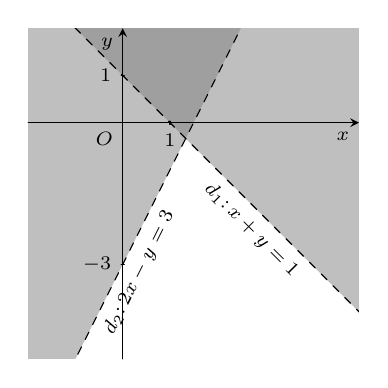
\begin{tikzpicture}[line join=round, line cap=round,>=stealth,font=\scriptsize, scale=0.6]
		\tikzset{label style/.style={font=\scriptsize}}
		\begin{scope}
			\clip (-2,-5) rectangle (5,2);
			\fill[gray, opacity =.5] (-6,-15)--(-6,9)--(6,9)--cycle;
			%\fill[pattern=north east lines] (-6,-15)--(-6,9)--(6,9)--cycle;
			\fill[gray, opacity =.5] (-6,7)--(7,7)--(7,-6)--cycle;
			\draw [dashed](4,5)--(-1,-5) node [pos=0.8, below, sloped] {$d_2\colon 2x -y=3$};
			\draw [dashed](-4,5)--(6,-5) node [pos=0.7, below, sloped] {$d_1\colon x+y =1$};
		\end{scope}
		\draw[->] (-2,0)--(5,0) node[below left]{$x$};
		\draw[->] (0,-5)--(0,2) node[below left]{$y$};
		\draw (0,0) node[below left]{$O$};
		\foreach \x in {1}
		\draw[thin] (\x,1pt)--(\x,-1pt) node [below] {$\x$};
		\foreach \y in {1,-3}
		\draw[thin] (1pt,\y)--(-1pt,\y) node [left] {$\y$};
	\end{tikzpicture}
	}
\loigiai{
	\begin{itemize}
		\item Hai đường thẳng $d_1\colon x+y =1$, $d_2\colon 2x -y=3$ đều biểu diễn cho biên của miền nghiệm hai bất phương trình.
		\item Điểm $O(0;0)$ không thuộc miền nghiệm của hệ bất phương trình.
		\item Hệ bất phương trình không tính biên nên các bất phương trình không có kèm dấu \lq\lq=\rq\rq.
	\end{itemize}
	Vậy miền nghiệm đã cho là miền nghiệm của hệ bất phương trình $\heva{&x+y<1\\&2x-y> 3}$
	}
\end{vd}
\begin{vd}%[0D2H2-2]%[Biên soạn tài liệu dạy học bộ KNTT-CS]%[Trịnh Ngọc Minh]
	Biểu diễn hình học tập nghiệm của hệ bất phương trình bậc nhất hai ẩn sau
	$$\heva{
	&2x+y \geq 2\\
	&x-2y \leq 1\\
	&y \leq 2\\
	&x \leq 3.}
	$$
	\loigiai
	{
	Vẽ các đường thẳng\\
	$d_1\colon 2x+y=2$;\\
	$d_2\colon x-2y=1$;\\
	$d_3\colon y=2$;\\
	$d_4\colon x=3$.
	\begin{center}
		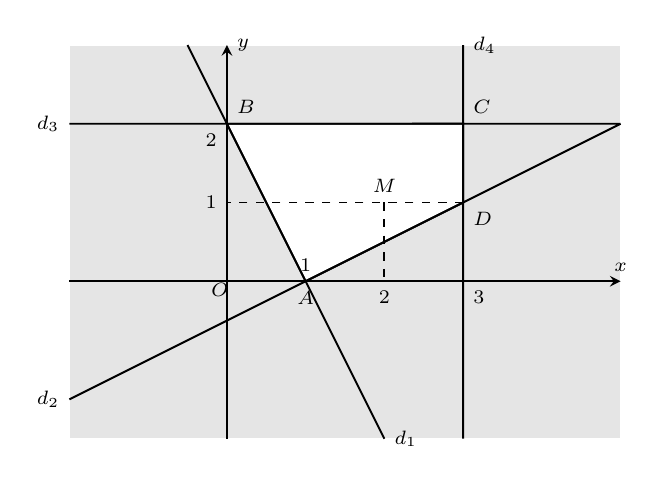
\begin{tikzpicture}[>=stealth,line width=0.7pt]
			\draw[color=white,fill=black!10] (-2,-2) rectangle (5,3);
			\path (-1/2,3) coordinate (A1);
			\path (2,-2) coordinate (B1);
			\path (-2,-3/2) coordinate (A2);
			\path (5,2) coordinate (B2);
			\path (-2,2) coordinate (A3);
			\path (5,2) coordinate (B3);
			\path (3,-2) coordinate (A4);
			\path (3,3) coordinate (B4);
			\path (intersection of A1--B1 and A2--B2) coordinate (A);
			\path (intersection of A1--B1 and A3--B3) coordinate (B);
			\path (intersection of A3--B3 and A4--B4) coordinate (C);
			\path (intersection of A2--B2 and A4--B4) coordinate (D);
			\draw[fill=white] (A) -- (B) -- (C) -- (D) -- cycle;
			\draw[->] (0,-2) -- (0,3) node[right]{\scriptsize $y$};
			\draw[->] (-2,0) -- (5,0) node[above]{\scriptsize $x$};
			\draw (0.15,0.1) node[below left]{\scriptsize $O$};
			\draw (A1) -- (B1) node[right]{\scriptsize $d_1$} (A2)node[left]{\scriptsize $d_2$} -- (B2) (A3)node[left]{\scriptsize $d_3$} -- (B3) (A4) -- (B4) node[right]{\scriptsize $d_4$};
			\draw[dashed] (A) node[above]{\scriptsize $1$} (A) node[below]{\scriptsize $A$} (B) node[below left]{\scriptsize $2$} (B) node[above right]{\scriptsize $B$} (C) node[above right]{\scriptsize $C$} (C|- 0,0) node[below right]{\scriptsize $3$} (D) node[below right]{\scriptsize $D$} -- (D-| 0,0) node[left]{\scriptsize $1$} (2,1) node[above]{\scriptsize $M$} -- (2,0)node[below]{\scriptsize $2$};
		\end{tikzpicture}
	\end{center}
	Vì điểm $M(2;1)$ có tọa độ thỏa mãn các bất phương trình trong hệ nên ta tô đậm các nửa mặt phẳng bờ $d_1$, $d_2$, $d_3$, $d_4$ không chứa $M$. Miền không bị tô đậm trong hình vẽ là miền nghiệm của hệ đã cho bao gồm các đoạn thẳng xác định miền.
	}
\end{vd}
\begin{vd}%[0D2H2-2]%[Biên soạn tài liệu dạy học bộ KNTT-CS]%[Trịnh Ngọc Minh]
	Biểu diễn miền nghiệm của hệ bất phương trình $\heva{&x+y\leq 0\\&\left|x \right| \leq 3.}$
\loigiai{
	\begin{itemize}
		\item 	Miền nghiệm của bất phương trình $x+y\leq 0$ là nửa mặt phẳng có bờ là đường thẳng $d_1 \colon x+y=0$ và không chứa điểm $ A(1;1) $, kể cả đường thẳng $d_1$, phần không gạch sọc.
		\item 	Miền nghiệm của bất phương trình $\left|x \right| \leq 3$ là phần mặt phẳng nằm giữa hai đường thẳng $d_2 \colon x=3$ và $d_3 \colon x=-3$ kể cả hai đường thẳng $d_2$ và $d_3$, phần không gạch sọc.
	\end{itemize}
	\begin{center}
		\begin{tikzpicture}[>=stealth,x=1cm,y=1cm,scale=0.5]
			%							\draw[color=gray,dash pattern=on 1pt off 1pt,xstep=1.0cm,ystep=1.0cm] (-5.2,-5.2) grid (5.2,5.2);
			\draw[->] (-5,0) -- (5,0) node[below] {\scriptsize $x$};
			\draw[->] (0,-5) -- (0,5) node[left] {\scriptsize $y$};
			\draw (0,0)node[below left]{\scriptsize $O$};
			\node at (1,-2) [right]{$d_1$};
			\node at (3,-4) [left]{$d_2$};
			\node at (-3,-4) [right]{$d_3$};
			\clip (-5,-5)rectangle(5,5);
			\draw[thick,samples=150,smooth,domain=-5:5] plot(\x,{(-1)*\x});
			\fill[pattern = north west lines,pattern color = violet!50, smooth,opacity=0.5] (-5,5)--(5,5)--(5,-5);
			\draw[thick] (3,-5)--(3,5);
			\fill[pattern = north west lines,pattern color = orange!50, smooth,opacity=0.5] (5,-5)--(3,-5)--(3,5)--(5,5);
			\draw[thick] (-3,-5)--(-3,5);
			\fill[pattern = north west lines,pattern color = orange!50, smooth,opacity=0.5] (-5,-5)--(-3,-5)--(-3,5)--(-5,5);
		\end{tikzpicture}
	\end{center}
	Vậy miền nghiệm của hệ bất phương trình là miền không gạch sọc và một phần các đường thẳng $d_1$, $d_2$, $d_3$.
	}
\end{vd}
\begin{dang}{Ứng dụng hệ bất phương trình bậc nhất hai ẩn giải bài toán tối ưu}
	Để tìm giá trị lớn nhất, nhỏ nhất của bài toán tối ưu ta thực hiện các bước sau\\
	\textbf{Bước 1.} Xác định miền nghiệm của hệ bất phương trình đã cho. Kết quả thường thu được là một đa giác.\\
	\textbf{Bước 2.} Tìm tọa độ đỉnh các đa giác. Tính giá trị $ T $ tương ứng với $ (x ; y) $ là tọa độ của các đỉnh của đa giác.\\
	\textbf{Bước 3.} Kết luận\\
	Giá trị lớn nhất hoặc nhỏ nhất của $ T $ là số lớn nhất hoặc nhỏ nhất trong các giá trị tìm được.
\end{dang}
\begin{vd}%[0D2H2-3]%[Biên soạn tài liệu dạy học bộ KNTT-CS]%[Trịnh Ngọc Minh]
	Một trang trại cần thuê xe để vận chuyển một lúc $120$ con bò sữa và $30$ tấn thức ăn cho bò. Giá thuê một chiếc xe lớn là $500$ nghìn đồng và một chiếc xe nhỏ là $350$ nghìn đồng. Gọi $x$ và $y$ lần lượt là số chiếc xe lớn và xe nhỏ mà chủ trang trại thuê. Xác định biểu thức biểu diễn tổng chi phí thuê xe (đơn vị: nghìn đồng)?
\loigiai{
	Vì mỗi xe lớn có giá $500$ nghìn đồng và mỗi xe nhỏ có giá $350$ nghìn đồng nên tổng chi phí thuê $x$ xe lớn và $y$ xe nhỏ là
	\[
	T=500x+350y \text{ (nghìn đồng).}
	\]
	}
\end{vd}
\begin{vd}%[0D2H2-3]%[Biên soạn tài liệu dạy học bộ KNTT-CS]%[Trịnh Ngọc Minh]
	Một cửa hàng dự định kinh doanh hai loại máy điều hòa: điều hòa một chiều và điều hòa hai chiều. Khảo sát thị trường cửa hàng thấy nhu cầu của thị trường sẽ không vượt quá $100$ máy cả hai loại. Gọi $x$, $y$ lần lượt là số máy điều hòa một chiều và điều hòa hai chiều mà cửa hàng nhập vào. Hãy lập hệ bất phương trình biểu diễn các điều kiện của bài toán.
\loigiai{
	Theo giả thiết, số máy điều hòa một chiều và hai chiều đều không âm nên $x\ge0$, $y\ge0$.  \\
	Do tổng số máy điều hòa không vượt quá $100$ máy nên $x+y\le100$. \\
	Vậy $(x;y)$ là nghiệm của hệ bất phương trình $\heva{&x\ge0\\&y\ge0\\&x+y\le100.}$
	}
\end{vd}
\begin{vd}%[0D2V2-3]%[Biên soạn tài liệu dạy học bộ KNTT-CS]%[Trịnh Ngọc Minh]
	Một người bán nước giải khát đang có $9$ lít nước, $14$ gam bột cam và $210$ gam đường để pha chế hai loại nước cam A và B. Để pha chế $1$ lít nước cam loại A cần $1$ lít nước, $1$ gam bột cam và $30$ gam đường; để pha chế $1$ lít nước cam loại B cần $1$ lít nước, $2$ gam bột cam và $10$ gam đường. Một lít nước cam loại A bán được $70$ nghìn đồng, mỗi lít nước cam loại B bán được $90$ nghìn đồng. Hỏi người đó đạt doanh thu cao nhất là bao nhiêu? Đơn vị tính là nghìn đồng.
\loigiai{
	Gọi $x$, $y$ lần lượt là số lít nước cam loại $A$ và $B$ cần pha chế.\\
	Ta có điều kiện $x\geq 0$; $y\geq 0$.\\
	Số lít nước cần sử dụng là $x+y\leq 9$;\\
	Số gam bột cam cần sử dụng là $x+2y\leq 14$;\\
	Số gam đường cần sử dụng là $3x+y\leq 21$.\\
	Ta có hệ bất phương trình
	$$\heva{&x+y\leq 9\\&x+2y\leq 14\\&3x+y\leq 21\\&x\geq 0\\&y\geq 0.}$$
	Biểu diễn từng miền nghiệm của bất phương trình trong hệ ta được miền nghiệm của hệ là miền ngũ giác $OABCD$ với $O(0;0)$, $A(0;7)$, $B(4;5)$, $C(6;3)$, $D(7;0)$.
	\begin{center}
		\begin{tikzpicture}[scale=0.6, font=\footnotesize, line join=round, line cap=round, >=stealth]
			\draw[-stealth] (-1,0)--(10,0) node [below] {$x$};
			\draw[-stealth] (0,-1)--(0,10) node [right] {$y$};
			\fill[pattern = north west lines,pattern color = black, smooth,opacity=0.5] (-1,-1)--(9.5,-1)--(9.5,9.5)--(-1,9.5);
			\foreach \y in {3,5,7}
			\draw (1pt,\y)--(-1pt,\y) node [left] {$\y$};
			\foreach \y in {1,2,4,6,8,9}
			\draw (1pt,\y)--(-1pt,\y);
			\foreach \x in {4,6,7}
			\draw (\x,1pt)--(\x,-1pt)node [below] {$\x$};
			\foreach \x in {1,2,3,5,8,9}
			\draw (\x,1pt)--(\x,-1pt);
			\path
			(0,0) coordinate (O)
			(0,7) coordinate (A)
			(4,5) coordinate (B)
			(6,3) coordinate (C)
			(7,0) coordinate (D)
			($(B)!1.2!(A)$) coordinate (a)
			($(A)!2.3!(B)$) coordinate (b)
			($(B)!2.7!(C)$) coordinate (p)
			($(C)!3.1!(B)$) coordinate (q)
			($(D)!3!(C)$) coordinate (c)
			($(C)!1.1!(D)$) coordinate (d);
			\draw[fill=white] (O)--(A)--(B)--(C)--(D)--cycle;
			\draw[dashed] (0,5)--(B)--(4,0) (0,3)--(C)--(6,0);
			\draw (a)--(b) (p)--(q) (d)--(c);
			\foreach \i/\j in {A/45, O/-135, B/45, C/45, D/45}\draw (\i) circle (1pt)++(\j:0.3) node {$\i$};
		\end{tikzpicture}
	\end{center}
	Doanh thu được tính theo biểu thức $F(x,y)=70x+90y $ (nghìn đồng). Ta có
	$$F(O)=70 \cdot 0+90\cdot 0=0,\ F(A)=70\cdot 0+90\cdot 7=630,$$
	$$F(B)=70\cdot 4+90\cdot 5=730,\ F(C)=70\cdot 6+90\cdot 3=690,\ F(D)=70\cdot 7+90\cdot 0=490.$$
	Vậy người đó nên pha $4$ lít nước cam loại $A$ và $5$ lít cam loại $B$ để có doanh thu cao nhất.
	}
\end{vd}
\subsection{BÀI TẬP RÈN LUYỆN}
%-------------Trắc nghiệm nhiều lựa chọn
\ind{PHẦN I.} \inden{Câu trắc nghiệm nhiều phương án lựa chọn. Mỗi câu hỏi học sinh chỉ chọn một phương án.}
\setcounter{ex}{0}
\Opensolutionfile{ans}[ans/ans-c2b4-lc]
\begin{ex}%[0D2N2-1]%[Biên soạn tài liệu dạy học bộ KNTT-CS]%[Trịnh Ngọc Minh]
	Cặp số nào là một nghiệm của hệ bất phương trình $\heva{&x-2y<5\\&3x+2y>6}$?
	\choice
	{$(5;0)$}
	{$(2;-2)$}
	{$(0;3)$}
	{\True $(5;3)$}
\loigiai{
	Cặp số $(5;3)$ thoả mãn cả hai bất phương trình của hệ đã cho nên $(5;3)$ là một nghiệm của hệ bất phương trình đó.
	}
\end{ex}
\begin{ex}%[0D2H2-1]%[Biên soạn tài liệu dạy học bộ KNTT-CS]%[Trịnh Ngọc Minh]
	Hệ bất phương trình $\heva{&5x - 3(y - x + 5) > 0 \\ &3x - 3(y - 5x + 5) \leq 0}$ tương đương với hệ bất phương trình nào sau đây?
	\choice
	{\True $\heva{&8 x - 3 y - 15 > 0 \\ &18 x - 3 y - 15 \leq 0}$}
	{$ \heva{&9 x - 3 y - 19 > 0 \\ &19 x - 3 y - 18 \leq 0} $}
	{$ \heva{&8 x - 2 y - 19 > 0 \\ &18 x - 2 y - 19 \leq 0} $}
	{$ \heva{&2 x + 3 y - 11 > 0 \\ &- 12 x + 3 y - 11 \leq 0} $}
\loigiai{
	Ta có hệ bất phương trình
	$$\heva{&5x - 3(y - x + 5) > 0 \\ &3x - 3(y - 5x + 5) \leq 0} \Leftrightarrow \heva{&8 x - 3 y - 15 > 0 \\ &18 x - 3 y - 15 \leq 0.}$$
	}
\end{ex}
\begin{ex}%[0D2N2-1]%[Biên soạn tài liệu dạy học bộ KNTT-CS]%[Trịnh Ngọc Minh]
	Hệ bất phương trình nào sau đây là hệ bất phương trình bậc nhất hai ẩn?
	\choice
	{$\heva{&x^2+y<0\\&y \ge 1}$}
	{\True $\heva{&x+y<0\\&y \ge 1}$}
	{$\heva{&x+y<0\\&y+z \ge 1}$}
	{$\heva{&x+y<0\\&y^2 \ge 1}$}
\loigiai{
	Chỉ có $\heva{&x+y<0\\&y \ge 1}$ là hệ bất phương trình bậc nhất hai ẩn.
	}
\end{ex}
\begin{ex}%[0D2H2-1]%[Biên soạn tài liệu dạy học bộ KNTT-CS]%[Trịnh Ngọc Minh]
	Điểm nào dưới đây \textbf{không} thuộc miền nghiệm của hệ bất phương trình $\heva{&x-1>0\\&x\geq 2y-4\\&y+x-2\leq 0}$?
	\choice
	{$(3;-5)$}
	{$(3;-3)$}
	{$(2;-1)$}
	{\True $(-1;-1)$}
\loigiai{
	Ta thấy $-1-1=-2>0$ (sai) nên cặp số $(-1;-1)$ không thuộc miền nghiệm của hệ bất phương trình đã cho.
	}
\end{ex}
\begin{ex}%[0D2H2-2]%[Biên soạn tài liệu dạy học bộ KNTT-CS]%[Trịnh Ngọc Minh]
	\immini[thm]{Cho hệ bất phương trình bậc nhất hai ẩn có miền nghiệm được biểu diễn như hình vẽ (phần không bị gạch, kể cả bờ).
	Điểm nào sau đây {\bfseries không} thuộc miền nghiệm của hệ bất phương trình đã cho?
	\choice
	{$(0;3)$}
	{$(0;0)$}
	{\True $(3;3)$}
	{$(3;-1)$}}{
	\begin{tikzpicture}[scale=0.7,>=stealth, font=\footnotesize, line join=round, line cap=round,declare function={k=1;f(\x)=-(\x)+3;g(\x)=-(\x)/9-1;h(\x)=(\x)+3;},xscale=k,yscale=k]
		\fill[pattern=north east lines,opacity=0.8] (-1,{f(-1)})--(5.5,{f(5.5)})--(5.5,{f(-1)})--cycle;
		\fill[pattern=north east lines,opacity=0.8] (-4.5,{g(-4.5)})--(5.5,{g(5.5)})--(5.5,{f(5.5)})--(-4.5,{f(5.5)})--cycle;
		\fill[pattern=north west lines,opacity=0.8] (-4.5,{h(-4.5)})--(1,{h(1)})--(-4.5,{h(1)})--cycle;
		\draw[->] (-5,0)--(5.5,0)node[fill=white,shift={(-120:.32)},scale=1]{$x$};
		\draw[->] (0,-2.5)--(0,4)node[fill=white,shift={(220:.36)},scale=1]{$y$};
		\path (0,0)coordinate(O) node[shift={(-135:.25)},scale=1]{$O$};
		\draw[violet,samples=100,domain=-1:5.5] plot (\x,{f(\x)});
		\draw[violet,samples=100,domain=-4.5:5.5] plot (\x,{g(\x)});
		\draw[violet,samples=100,domain=-4.5:1] plot (\x,{h(\x)});
		\path (4,{f(4)}) node[shift={(180:.3)},scale=1]{$d_1$};
		\path (1.5,{g(1)}) node[shift={(80:.3)},scale=1]{$d_2$};
		\path (-1,{h(-1)}) node[shift={(-70:.3)},scale=1]{$d_3$};
		\foreach \i/\g in {-1/30,3/180}{\draw[fill=black](0,\i) circle (1pt) ($(0,\i)+(\g:3mm)$) node[scale=1]{$\i$};}
		\foreach \i/\g in {-3/-90,3/-90}{\draw[fill=black](\i,0) circle (1pt) ($(\i,0)+(\g:3mm)$) node[scale=1]{$\i$};}
	\end{tikzpicture}
	}
\loigiai{
	Theo hình biểu diễn miền nghiệm của hệ bất phương trình, ta có các điểm $(0;3)$, $(0;0)$, $(3;-1)$ thuộc miền nghiệm của hệ bất phương trình. Còn điểm $(3;3)$ không thuộc miền nghiệm của hệ bất phương trình.
	}
\end{ex}
\begin{ex}%[0D2H2-1]%[Biên soạn tài liệu dạy học bộ KNTT-CS]%[Trịnh Ngọc Minh]
	Trong các hệ sau đây, có bao nhiêu hệ bất phương trình bậc nhất hai ẩn?
	\begin{listEX}[2]
		\item $\heva{&3x+y-1 \leq 0\\ &2x-y+2 \geq 0}$.
		\item $\heva{&5 x+y-9=0\\&4 x-7y+3=0}$.
		\item $\heva{&y-1<0\\&x+2 \geq 0}$.
		\item $\heva{&x+y-3 \leq 0\\ &-2x+y+3 \geq 0\\&x \geq 0\\ &y \geq 0}$.
	\end{listEX}
	\choice
	{\True $3$}
	{$2$}
	{$1$}
	{$0$}
\loigiai{
	Các hệ a), c), d) là các hệ bất phương trình bậc nhất hai ẩn.\\
	Hệ b) không phải hệ bất phương trình bậc nhất hai ẩn vì hệ này gồm các phương trình.
	}
\end{ex}
\begin{ex}%[0D2H2-1]%[Biên soạn tài liệu dạy học bộ KNTT-CS]%[Trịnh Ngọc Minh]
	Hệ bất phương trình $\heva{&3x-y+3>0\\ &-2x+3y-6<0\\ &2x+y+4>0}$ có một nghiệm là
	\choice
	{$(-2;2)$}
	{$(-2;-2)$}
	{\True $(1;-2)$}
	{$(-1;2)$}
	\loigiai
	{
	Thế $(1;-2)$ vào từng bất phương trình của hệ ta có
	\begin{itemize}
		\item $3\cdot 1-(-2)+6>0$ (đúng).
		\item $-2\cdot 1+3(-2)-6<0$ (đúng).
		\item $2\cdot 1+(-2)+4>0$ (đúng).
	\end{itemize}
	Vậy $(1;-2)$ là một nghiệm của hệ bất phương trình.
	}
\end{ex}
\begin{ex}%[0D2H2-2]%[Biên soạn tài liệu dạy học bộ KNTT-CS]%[Trịnh Ngọc Minh]
	Miền nghiệm của hệ bất phương trình $\heva{&x-2y<0\\ &x+3y>-2\\ &y-x<3}$ là phần \textbf{không} tô đậm của hình vẽ nào trong các hình vẽ sau?
	\choice
	{\begin{tikzpicture}[line join=round, line cap=round, >=stealth,font=\footnotesize, scale=0.4]
	% Vẽ hệ trục toạ độ
	\draw (0,0) node [right] {$O$};
	\draw [->] (-6.5,0)--(4.5,0) node[below]{$x$};
	\draw[->] (0,-6.5)--(0,4.5) node[left]{$y$};
	\clip(-6.5,-4.5) rectangle (4.5,4.5);
	% Vẽ các số trên hai trục
	\foreach \x in {-3,-2}
	\draw[shift={(\x,0)},color=black] (0pt,2pt) -- (0pt,-2pt) node[below] {$\x$};
	\foreach \y in {3}
	\draw[shift={(0,\y)},color=black] (2pt,0pt) -- (-2pt,0pt)node[right] {$\y$};
	%Vẽ đồ thị từng hàm số
	\draw[samples=100,smooth,domain=-6.5:4.5,black] plot(\x,{0.5*(\x)});
	\draw[samples=100,smooth,domain=-6.5:4.5,black] plot(\x,{-1/3*(\x)-2/3});
	\draw[samples=100,smooth,domain=-6.5:4.5,black] plot(\x,{(\x)+3});
	% Vẽ miền nghiệm
	\fill[pattern=north west lines,opacity=0.6] plot[domain=-6.5:4.5](\x,{(\x)+3})--plot[domain=4.5:-6.5](\x,{4.5})--cycle;
	\fill[pattern=north west lines,opacity=0.6] plot[domain=-6.5:4.5](\x,{-1/3*(\x)-2/3})--plot[domain=4.5:-6.5](\x,{4.5})--cycle;
	\fill[pattern=north west lines,opacity=0.6] plot[domain=-6.5:4.5](\x,{0.5*(\x)})--plot[domain=4.5:-6.5](\x,{4.5})--cycle;
	\end{tikzpicture}}
	{\True \begin{tikzpicture}[line join=round, line cap=round, >=stealth,font=\footnotesize, scale=0.4]
	% Vẽ hệ trục toạ độ
	\draw (0,0) node [right] {$O$};
	\draw [->] (-6.5,0)--(4.5,0) node[below]{$x$};
	\draw[->] (0,-6.5)--(0,4.5) node[left]{$y$};
	\clip(-6.5,-4.5) rectangle (4.5,4.5);
	% Vẽ các số trên hai trục
	\foreach \x in {-3,-2}
	\draw[shift={(\x,0)},color=black] (0pt,2pt) -- (0pt,-2pt) node[below] {$\x$};
	\foreach \y in {3}
	\draw[shift={(0,\y)},color=black] (2pt,0pt) -- (-2pt,0pt)node[right] {$\y$};
	%Vẽ đồ thị từng hàm số
	\draw[samples=100,smooth,domain=-6.5:4.5,black] plot(\x,{0.5*(\x)});
	\draw[samples=100,smooth,domain=-6.5:4.5,black] plot(\x,{-1/3*(\x)-2/3});
	\draw[samples=100,smooth,domain=-6.5:4.5,black] plot(\x,{(\x)+3});
	% Vẽ miền nghiệm
	\fill[pattern=north west lines,opacity=0.6] plot[domain=-6.5:4.5](\x,{(\x)+3})--plot[domain=4.5:-6.5](\x,{4.5})--cycle;
	\fill[pattern=north west lines,opacity=0.6] plot[domain=-6.5:4.5](\x,{-1/3*(\x)-2/3})--plot[domain=4.5:-6.5](\x,{-6.5})--cycle;
	\fill[pattern=north west lines,opacity=0.6] plot[domain=-6.5:4.5](\x,{0.5*(\x)})--plot[domain=4.5:-6.5](\x,{-6.5})--cycle;
	\end{tikzpicture}}
	{\begin{tikzpicture}[line join=round, line cap=round, >=stealth,font=\footnotesize, scale=0.4]
	% Vẽ hệ trục toạ độ
	\draw (0,0) node [right] {$O$};
	\draw [->] (-6.5,0)--(4.5,0) node[below]{$x$};
	\draw[->] (0,-6.5)--(0,4.5) node[left]{$y$};
	\clip(-6.5,-4.5) rectangle (4.5,4.5);
	% Vẽ các số trên hai trục
	\foreach \x in {-3,-2}
	\draw[shift={(\x,0)},color=black] (0pt,2pt) -- (0pt,-2pt) node[below] {$\x$};
	\foreach \y in {3}
	\draw[shift={(0,\y)},color=black] (2pt,0pt) -- (-2pt,0pt)node[right] {$\y$};
	%Vẽ đồ thị từng hàm số
	\draw[samples=100,smooth,domain=-6.5:4.5,black] plot(\x,{0.5*(\x)});
	\draw[samples=100,smooth,domain=-6.5:4.5,black] plot(\x,{-1/3*(\x)-2/3});
	\draw[samples=100,smooth,domain=-6.5:4.5,black] plot(\x,{(\x)+3});
	% Vẽ miền nghiệm
	\fill[pattern=north west lines,opacity=0.6] plot[domain=-6.5:4.5](\x,{(\x)+3})--plot[domain=4.5:-6.5](\x,{-6.5})--cycle;
	\fill[pattern=north west lines,opacity=0.6] plot[domain=-6.5:4.5](\x,{-1/3*(\x)-2/3})--plot[domain=4.5:-6.5](\x,{4.5})--cycle;
	\fill[pattern=north west lines,opacity=0.6] plot[domain=-6.5:4.5](\x,{0.5*(\x)})--plot[domain=4.5:-6.5](\x,{-6.5})--cycle;
	\end{tikzpicture}}
	{\begin{tikzpicture}[line join=round, line cap=round, >=stealth,font=\footnotesize, scale=0.4]
	% Vẽ hệ trục toạ độ
	\draw (0,0) node [right] {$O$};
	\draw [->] (-6.5,0)--(4.5,0) node[below]{$x$};
	\draw[->] (0,-6.5)--(0,4.5) node[left]{$y$};
	\clip(-6.5,-4.5) rectangle (4.5,4.5);
	% Vẽ các số trên hai trục
	\foreach \x in {-3,-2}
	\draw[shift={(\x,0)},color=black] (0pt,2pt) -- (0pt,-2pt) node[below] {$\x$};
	\foreach \y in {3}
	\draw[shift={(0,\y)},color=black] (2pt,0pt) -- (-2pt,0pt)node[right] {$\y$};
	%Vẽ đồ thị từng hàm số
	\draw[samples=100,smooth,domain=-6.5:4.5,black] plot(\x,{0.5*(\x)});
	\draw[samples=100,smooth,domain=-6.5:4.5,black] plot(\x,{-1/3*(\x)-2/3});
	\draw[samples=100,smooth,domain=-6.5:4.5,black] plot(\x,{(\x)+3});
	% Vẽ miền nghiệm
	\fill[pattern=north west lines,opacity=0.6] plot[domain=-6.5:4.5](\x,{(\x)+3})--plot[domain=4.5:-6.5](\x,{4.5})--cycle;
	\fill[pattern=north west lines,opacity=0.6] plot[domain=-6.5:4.5](\x,{-1/3*(\x)-2/3})--plot[domain=4.5:-6.5](\x,{4.5})--cycle;
	\fill[pattern=north west lines,opacity=0.6] plot[domain=-6.5:4.5](\x,{0.5*(\x)})--plot[domain=4.5:-6.5](\x,{-6.5})--cycle;
	\end{tikzpicture}}
\loigiai{
	Xét đường thẳng $d\colon x-2y=0 $.\\
	Thay tọa độ điểm $(-1;0)$ vào vế trái phương trình đường thẳng $(d)$, ta được $-1<0$.\\
	Vậy miền nghiệm của bất phương trình $x-2y<0$ là nửa mặt phẳng chứa điểm $(-1,0)$, không kể cả bờ $(d)$.\\
	Do chỉ có hình
	\begin{center}
		\begin{tikzpicture}[line join=round, line cap=round, >=stealth,font=\footnotesize, scale=0.4]
			% Vẽ hệ trục toạ độ
			\draw (0,0) node [right] {$O$};
			\draw [->] (-6.5,0)--(4.5,0) node[below]{$x$};
			\draw[->] (0,-6.5)--(0,4.5) node[left]{$y$};
			\clip(-6.5,-4.5) rectangle (4.5,4.5);
			% Vẽ các số trên hai trục
			\foreach \x in {-3,-2}
			\draw[shift={(\x,0)},color=black] (0pt,2pt) -- (0pt,-2pt) node[below] {$\x$};
			\foreach \y in {3}
			\draw[shift={(0,\y)},color=black] (2pt,0pt) -- (-2pt,0pt)node[right] {$\y$};
			%Vẽ đồ thị từng hàm số
			\draw[samples=100,smooth,domain=-6.5:4.5,black] plot(\x,{0.5*(\x)});
			\draw[samples=100,smooth,domain=-6.5:4.5,black] plot(\x,{-1/3*(\x)-2/3});
			\draw[samples=100,smooth,domain=-6.5:4.5,black] plot(\x,{(\x)+3});
			% Vẽ miền nghiệm
			\fill[pattern=north west lines,opacity=0.6] plot[domain=-6.5:4.5](\x,{(\x)+3})--plot[domain=4.5:-6.5](\x,{4.5})--cycle;
			\fill[pattern=north west lines,opacity=0.6] plot[domain=-6.5:4.5](\x,{-1/3*(\x)-2/3})--plot[domain=4.5:-6.5](\x,{-6.5})--cycle;
			\fill[pattern=north west lines,opacity=0.6] plot[domain=-6.5:4.5](\x,{0.5*(\x)})--plot[domain=4.5:-6.5](\x,{-6.5})--cycle;
		\end{tikzpicture}
	\end{center}
	chứa điểm $(-1;0)$ nên ta chọn hình này.
	}
\end{ex}
\begin{ex}%[0D2H2-2]%[Biên soạn tài liệu dạy học bộ KNTT-CS]%[Trịnh Ngọc Minh]
	\immini[thm]{Phần gạch chéo trong hình bên là miền nghiệm của hệ bất phương trình nào dưới đây?
	\choice
	{\True $\heva{&2x+y \leq 4\\&x+y \leq 3\\ &x \geq 0\\ &y \geq 0}$}
	{$\heva{&2x+y \geq 4\\&x+y \leq 3\\ &x \geq 0\\ &y \geq 0}$}
	{$\heva{&2x+y \leq 4\\&x+y \geq 3\\ &x \geq 0\\ &y \geq 0}$}
	{$\heva{&2x+y \leq 4\\&x+y \leq 3\\ &x \geq 0\\ &y<0}$}}{
	\begin{tikzpicture}[scale=0.8,>=stealth, font=\footnotesize, line join=round,line width=1pt, line cap=round]
		\def\a{-1} \def\b{0} \def\c{1} \def\d{1} % Hệ số
		\def\xmin{-1} \def\xmax{4}
		\def\ymin{-1} \def\ymax{5}
		\draw[->] (\xmin,0)--(\xmax,0) node [below]{$x$};
		\draw[->] (0,\ymin)--(0,\ymax) node [left]{$y$};
		\draw[smooth,samples=300,domain=-1:4] plot(\x,{3-\x});
		\draw[smooth,samples=300,domain=-0.8:3] plot(\x,{4-2*(\x)});
		\fill (0,3)node[left]{$3$} circle (1.5pt);
		\fill (0,4)node[left]{$4$}circle (1.5pt);
		\fill (3,0)node[below]{$3$}circle (1.5pt);
		\fill (2,0)node[below]{$2$}circle (1.5pt);
		\fill (1,2)circle (1.5pt);
		\fill [pattern =north east lines ] (0,0)--(0,3)--(1,2)--(2,0)--(0,0);
	\end{tikzpicture}
	}
\loigiai{
	Dựa vào hình vẽ ta thấy miền nghiệm được giới hạn bởi các đường thẳng $2x+y=4$; $x+y=3$; $x=0$; $y=0$.\\
	Miền nghiệm gồm các điểm có hoành độ $x \geq 0$ và tung độ $y \geq 0$.\\
	Lại có điểm $(1; 1)$ thuộc miền nghiệm thỏa mãn bất phương trình $2x+y \leq 4;x+y \leq 3$.
	}
\end{ex}
\begin{ex}%[0D2H2-2]%[Biên soạn tài liệu dạy học bộ KNTT-CS]%[Trịnh Ngọc Minh]
	\immini[thm]{Phần không gạch chéo ở hình sau đây là biểu diễn miền nghiệm của hệ bất phương trình?
	\choice
	{$\heva{&x>0\\&3x+2y>-6}$}
	{\True $\heva{&y\geq 0\\&3x+2y<6}$}
	{$\heva{&y>0\\&3x+2y<-6}$}
	{$\heva{&x>0\\&3x+2y<6}$}
	}{
	\begin{tikzpicture}[scale=0.8,font=\footnotesize,line join=round,line cap=round,>=stealth]
		\begin{scope}
			\clip (-1,-1) rectangle (3,4);
			\fill[opacity=.5,pattern=north east lines] (-2.3,-2)--(4,-2)--(4,0)--(-2.3,0)--cycle;
			\fill[opacity=.5,pattern=north east lines] (-0.6,4)--(2,0)--(4,0)--(4,4)--cycle;
			\draw[smooth,samples=200] plot[domain=-0.6:3.2] (\x,{-3/2*\x+3});
		\end{scope}
		\draw[->] (-1,0)--(3,0)node[below]{$x$};
		\draw[->] (0,-1)--(0,4)node[below right]{$y$};
		\draw (0,0)node[below left]{$O$};
		\foreach \x in {2}
		\draw[thin] (\x,1pt)--(\x,-1pt) node [above] {$\x$};
		\foreach \y in {3}
		\draw[thin] (1pt,\y)--(-1pt,\y) node [left] {$\y$};
	\end{tikzpicture}}
\loigiai{
	Xét điểm $A(0;1)$ thuộc miền nghiệm của hệ bất phương trình. Khi đó, ta thay tọa độ điểm $A$ lần lượt vào các hệ bất phương trình kiểm tra thì
	\begin{itemize}
		\item $\heva{&1\ge 0\\ &3\cdot 0+2\cdot 1=2<6}$ thỏa mãn hệ bất phương trình $\heva{&y\geq 0\\&3x+2y<6.}$
		\item $\heva{&1>0\\ &3\cdot 0+2\cdot 1=2>-6}$ không thỏa mãn hệ bất phương trình $\heva{&y>0\\&3x+2y<-6.}$
		\item $\heva{&0>0 \text{(vô lí)}\\ &3\cdot 0+2\cdot 1=2<6}$ không thỏa mãn hệ bất phương trình $\heva{&x>0\\&3x+2y<6.}$
		\item $\heva{&0>0 \text{(vô lí)}\\ &3\cdot 0+2\cdot 1=2>-6}$ không thỏa mãn hệ bất phương trình $\heva{&x>0\\&3x+2y>-6.}$
	\end{itemize}
	Vậy hệ bất phương trình $\heva{&y\geq 0\\&3x+2y<6}$ biểu diễn miền nghiệm của hình vẽ.
	}
\end{ex}
\begin{ex}%[0D2N1-3]%[Biên soạn tài liệu dạy học bộ KNTT-CS]%[Trịnh Ngọc Minh]
	Một gia đình cần ít nhất $2{,}3$\,kg protein và $1{,}2$\,kg lipit mỗi ngày. Biết rằng thịt gà chứa $25\%$ protein và $20\%$ lipit; thịt cá chứa $20\%$ protein và $10\%$ lipit. Giá tiền $1$\,kg thịt gà là $80\,000$ đồng và $1$\,kg thịt cá là $110\,000$ đồng. Giả sử gia đình mua $x$\,kg thịt gà và $y$\,kg thịt cá. Biểu thức nào sau đây biểu thị tổng chi phí (tính bằng nghìn đồng) để mua số thịt đó?
	\choice
	{\True $T=80x+110y$}
	{$T=110x+80y$}
	{$T=0{,}8x+1{,}1y$}
	{$T=8x+11y$}
\loigiai{
	Do giá $1$\,kg thịt gà là $80$ nghìn đồng và $1$\,kg thịt cá là $110$ nghìn đồng nên tổng chi phí khi mua $x$\,kg thịt gà và $y$\,kg thịt cá là
	\[
	T=80x+110y \text{ (nghìn đồng).}
	\]
	}
\end{ex}
\begin{ex}%[0D2H2-3]%[Biên soạn tài liệu dạy học bộ KNTT-CS]%[Trịnh Ngọc Minh]
	Bác An dự định để $x$ sào đất trồng cà tím và $y$ sào đất trồng cà chua. Bác dự định để tối đa $10$ triệu đồng để mua hạt giống. Tiền mua hạt giống cà tím là $200\,000$ đồng/sào và cà chua là $100\,000$ đồng/sào. Hệ phương trình mô tả điều kiện của $x$, $y$ là
	\choice
	{\True $\heva{&2x+y\le 100\\ &x\ge 0\\ &y\ge 0}$}
	{$\heva{&2x+y\le 1\,000\\ &x\ge 0\\ &y\ge 0}$}
	{$\heva{&x+2y\le 100\\ &x\ge 0\\ &y\ge 0}$}
	{$\heva{&2x+y\ge 100\\ &x\ge 0\\ &y\ge 0}$}
\loigiai{
	Diện tích đất trồng cà tím và cà chua là các số không âm nên $x\ge0$, $y\ge0$.\\
	Vì tiền mua hạt giống cà tím là $200\,000$ đồng/sào, cà chua là $100\,000$ đồng/sào và số tiền tối đa là $10$ triệu đồng nên $200\,000x+100\,000y\le 10\,000\,000$ $\Leftrightarrow$ $2x+y\le100$.\\
	Vậy hệ phương trình mô tả điều kiện của $x$, $y$ là $\heva{&2x+y\le 100\\ &x\ge 0\\ &y\ge 0.}$
	}
\end{ex}
\Closesolutionfile{ans}
\indapan{6}{ans/ans-c2b4-lc}
%---------------------Trắc nghiệm đúng sai
\ind{PHẦN II.} \inden{Câu trắc nghiệm đúng sai. Trong mỗi ý a), b), c), d) ở mỗi câu, học sinh chọn đúng hoặc sai.}
\setcounter{ex}{0}
\Opensolutionfile{ans}[ans/ans-c2b4-ds]
\begin{ex}%[0D2H2-2]%[Biên soạn tài liệu dạy học bộ KNTT-CS]%[Trịnh Ngọc Minh]
	Cho hệ bất phương trình $\heva{&2x+5y \geq 10\\ &4x+5y \leq 20\\ &2x+y \geq 4.}$
	\choiceTF
	{\True Điểm $M(2; 2)$ thuộc miền nghiệm của hệ bất phương trình đã cho}
	{Tọa độ của tất cả các điểm nằm trên đường thẳng $4x+5y=20$ đều là nghiệm của hệ bất phương trình đã cho}
	{\True Miền nghiệm của hệ bất phương trình đã cho là một miền tam giác}
	{Diện tích miền nghiệm của hệ bất phương trình đã cho bằng $3$}
\loigiai{
	\begin{itemchoice}
		\itemch Thay $x=2$; $y=2$ vào hệ bất bất phương trình đã cho ta được mệnh đề đúng.
		\itemch Ta có $4x+5y=20$ hay $ y=\dfrac{20-4x}{5}$, thay vào bất phương trình thứ ba trong hệ bất phương trình đã cho ta có $2x+\dfrac{20-4x}{5} \geq 4$ hay $ 6x \geq 0$ suy ra $ x \geq 0$.\\
		Do đó bất bất phương trình thứ ba trong hệ bất phương trình đã cho chỉ đúng với tọa độ các điểm nằm trên đường thẳng $4x+5y=20$ mà có hoành độ dương.
		\itemch Vẽ các đường thẳng $d_1\colon 2x+5y=10$; $d_2\colon 4x+5y=20$; $d_3\colon 2x+y=4$.\\
		Gạch đi các phần không thuộc miền nghiệm của mỗi bất phương trình trên
		\begin{center}\begin{tikzpicture}[scale=0.7,>=stealth, font=\footnotesize, line join=round,line width=1pt, line cap=round]
			\def\a{-1} \def\b{0} \def\c{1} \def\d{1} % Hệ số
			\def\xmin{-1} \def\xmax{6}
			\def\ymin{-1} \def\ymax{5.5}
			\draw[->] (\xmin,0)--(5,0)node[above]{$B$}--(\xmax,0) node [below]{$x$};
			\draw[->] (0,\ymin)--(0,4)node[right]{$C$}--(0,\ymax) node [left]{$y$};
			\draw[smooth,samples=300,domain=-1:5.8] plot(\x,{2-0.4*(\x)});
			\draw[smooth,samples=300,domain=-1:5.6] plot(\x,{4-0.8*(\x)});
			\draw[smooth,samples=300,domain=-0.8:2.5] plot(\x,{4-2*(\x)});
			\fill (0,2)node[above left]{$2$} circle (1.5pt);
			\fill (0,4)node[left]{$4$}circle (1.5pt);
			\fill (5,0)node[below]{$5$}circle (1.5pt);
			\fill (2,0)node[below]{$2$}circle (1.5pt);
			\fill (1.25,1.5)circle (1.5pt);
			\draw[dashed] (1.25,0)node[below]{$\dfrac{5}{4}$}--(1.25,1.5)node[below left]{$A$}--(0,1.5)node[left]{$\dfrac{3}{2}$};
			\fill [pattern =north east lines ] (-1,6)--(2.5,-1)--(-1,-1)--(-1,6);
			\fill [pattern =north east lines ] (-1,4.8)--(-1,6)--(6,6)--(6,-0.8)--(-1,4.8);
			\fill [pattern =north east lines ] (-1,2.4)--(-1,-1)--(6,-1)--(6,-0.4)--(-1,2.4);
			\end{tikzpicture}\end{center}
			Miền nhiệm của hệ bất phương trình đã cho là miền tam giác $ABC$ với $A\left(\dfrac{5}{4}; \dfrac{3}{2}\right)$; $B(5; 0)$; $C(0; 4)$
			\itemch Ta có $BC=\sqrt{41}$, $AB=\dfrac{3\sqrt{29}}{4}$, $AC=\dfrac{5\sqrt{5}}{4}$\\
			Áp dụng công thức Herong ta có $S_{ABC}=\dfrac{15}{4}=3{,}75$.
			\end{itemchoice}
			}
\end{ex}
\begin{ex}%[0D2H2-2]%[Biên soạn tài liệu dạy học bộ KNTT-CS]%[Trịnh Ngọc Minh]
	\immini[thm]{Phần \textbf{không} bị gạch (không kể bờ) trong hình vẽ bên biểu diễn miền nghiệm của một hệ bất phương trình bậc nhất hai ẩn.
	\choiceTF
	{Điểm $O(0;0)$ thuộc miền nghiệm của hệ bất phương trình đã cho}
	{\True Điểm $A(1;-1)$ thuộc miền nghiệm của hệ bất phương trình đã cho}
	{\True Điểm $B(1;0)$ thuộc miền nghiệm của hệ bất phương trình đã cho}
	{\True Miền nghiệm trong hình vẽ biểu diễn miền nghiệm của hệ bất phương trình $\heva{&x-y>0\\&2x-y>1}$
	} }{
	\begin{tikzpicture}[scale=1, font=\footnotesize, line join=round, line cap=round, >=stealth]
		\def\xmin{-2} \def\xmax{2.5}
		\def\ymin{-1.8} \def\ymax{2}
		\draw[->] (\xmin,0)--(\xmax,0) node [below]{$x$};
		\draw[->] (0,\ymin)--(0,\ymax) node [left]{$y$};
		\draw[dashed] (1,0)--(1,1)--(0,1);
		\fill (0,0)node[above left]{$O$} (1,0)node[below]{$1$}(0,1)node[left]{$1$}
		(0,-1)node[left]{$-1$}
		;
		\clip (\xmin+0.1,\ymin+0.1) rectangle (\xmax-0.1,\ymax-0.1);
		\draw[smooth,samples=300] plot(\x,{\x});
		\draw[smooth,samples=300] plot(\x,{2*\x-1});
		\fill[pattern=north east lines](-2,2)--(2.5,2)--(2,2)--(1,1)--(-0.5,-2)--(-2,-2)--cycle
		;
	\end{tikzpicture}
	}
\loigiai{
	\begin{itemchoice}
		\itemch Điểm $O(0;0)$ không thuộc miền nghiệm của hệ bất phương trình đã cho.
		\itemch Điểm $A(1;-1)$ thuộc miền nghiệm của hệ bất phương trình đã cho.
		\itemch Điểm $B(1;0)$ thuộc miền nghiệm của hệ bất phương trình đã cho.
		\itemch Miền nghiệm trong hình vẽ biểu diễn miền nghiệm của hệ bất phương trình $\heva{&x-y>0\\&2x-y>1}$
	\end{itemchoice}
	}
\end{ex}
\begin{ex}%[0D2H2-3]%[Biên soạn tài liệu dạy học bộ KNTT-CS]%[Trịnh Ngọc Minh]
	Ngoài giờ học, bạn Minh làm thêm việc phụ bán phở được $15$ nghìn đồng một giờ và phụ bán tạp hoá được $10$ nghìn đồng một giờ. Minh không thể làm việc nhiều hơn $16$ giờ mỗi tuần. Gọi $x$ và $y$ lần lượt là số giờ phụ bán phở và phụ bán hàng trong $1$ tuần.
	\choiceTF
	{\True Số tiền Minh kiếm thêm được trong $1$ tuần là $15x+10y$ (nghìn đồng)}
	{\True Số giờ làm thêm trong một tuần của Minh thoả mãn bất phương trình $x+y\le 16$}
	{\True Nếu trong $1$ tuần, Minh phụ bán phở $7$ giờ và phụ bán hàng $6$ giờ thì Minh sẽ kiếm được nhiều hơn $100$ nghìn đồng}
	{Hệ bất phương trình $\heva{&x\ge 0\\&y\ge 0\\&x+y\le 16\\&3x+2y\ge 10}$ biểu thị số giờ để làm mỗi việc nếu Minh muốn kiếm được ít nhất $100$ nghìn đồng mỗi tuần}
\loigiai{\begin{itemchoice}
	\itemch
	Vì bạn Minh làm thêm việc phụ bán phở được $15$ nghìn đồng/ $1$ giờ và phụ bán tạp hoá được $10$ nghìn đồng/ $1$ giờ nên số tiền Minh kiếm thêm được trong $1$ tuần là $15x+10y$ (nghìn đồng).
	\itemch
	Vì Minh không thể làm việc nhiều hơn $16$ giờ mỗi tuần nên số giờ làm thêm trong một tuần của Minh thoả mãn bất phương trình $x+y\le 16$.
	\itemch
	Nếu Minh phụ bán phở $7$ giờ và phụ bán hàng $6$ giờ thì số tiền Minh kiếm được là $15\cdot 7+10\cdot 6=165$ nghìn đồng.
	\itemch
	Để kiếm ít nhất $100$ nghìn đồng mỗi tuần thì $15x+10y\ge 100$. Suy ra $3x+2y\ge 20$.\\
	Vậy $\heva{&x\ge 0\\&y\ge 0\\&x+y\le 16\\&3x+2y\ge 20.}$
	\end{itemchoice}
	}
\end{ex}
\begin{ex}%[0D2V2-3]%[Biên soạn tài liệu dạy học bộ KNTT-CS]%[Trịnh Ngọc Minh]
	Trong một cuộc thi pha chế, mỗi đội chơi được sử dụng tối đa $ 24$\,g hương liệu, $ 9 $ lít nước và $ 210$\,g đường để pha chế nước cam và nước táo. Để pha chế $ 1 $ lít nước cam cần $ 30$\,g đường, $ 1 $ lít nước và $ 1$\,g hương liệu; pha chế $ 1 $ lít nước táo cần $ 10$\,g đường, $ 1 $ lít nước và $ 4$\,g hương liệu. Mỗi lít nước cam nhận được $ 60$ điểm thưởng, mỗi lít nước táo nhận được $ 80 $ điểm thưởng.
	Gọi $x$ và $y$ là số lít nước cam và nước táo cần pha chế để số điểm thưởng nhận được là lớn nhất.
	\choiceTF
	{\True Số điểm thưởng của đội là $60x+80y$}
	{\True Số gam đường cần dùng $30x+10y$}
	{\True Các giá trị $x$, $y$ thỏa mãn hệ bất phương trình $\heva{&3x+y\le 21\\&x+y\le 9\\ &x+4y\le 24\\&x,y\ge 0}$}
	{Số điểm thưởng lớn nhất mà đội nhận được là $600$ điểm}
\loigiai{
	Gọi $x$, $y $ lần lượt là số lít nước cam và táo của một đội pha chế $ (x,y\ge 0)$.
	\begin{itemchoice}
		\itemch Số điểm thưởng của đội chơi này là $ f(x;y)=60x+80y$.
		\itemch Số gam đường cần dùng là $ 30x+10y$.
		\itemch Thật vậy, ta tìm thêm các ràng buộc đối với $x$ và $y$.\\
		Số gam hương liệu cần dùng là $x+4y $.\\
		Tương tự ta có số lít nước cần dùng là $x+y$.\\
		Vì trong cuộc thi pha chế, mỗi đội chơi sử dụng tối đa $ 24 $\,g hương liệu, $ 9 $ lít nước và $ 210$\,g đường nên ta có hệ bất phương trình $\heva{&30x+10y\le 210\\&x+y\le 9\\ &x+4y\le 24\\&x,y\ge 0}$ hay $ \heva{&3x+y\le 21\\&x+y\le 9\\ &x+4y\le 24\\&x,y\ge 0.} \quad (*)$\\
		\itemch
		\immini{Bài toán trở thành tìm giá trị lớn nhất của hàm số $ f(x;y) $ trên miền nghiệm của hệ bất phương
		trình $ (*)$.\\
		Miền nghiệm của hệ bất phương trình $(*)$ là ngũ giác $ OABCD $ (kể cả biên).\\
		Hàm số $ f(x;y)=60x+80y $ sẽ đạt giá trị lớn nhất trên miền nghiệm của hệ bất phương trình $ (*) $ khi $ (x;y) $ là toạ độ của một trong các đỉnh $ O(0;0), A(7;0), B(6;3), C(4;5), D(0;6).$\\
		Ta có $ f(0;0)=0; f(7;0)=420; f(6;3)=600; f(4;5)=640; f(0;6)=480. $\\
		Suy ra $ f(4;5) $ là giá trị lớn nhất của hàm số $ f(x;y) $ trên miền nghiệm của hệ $ (*). $}{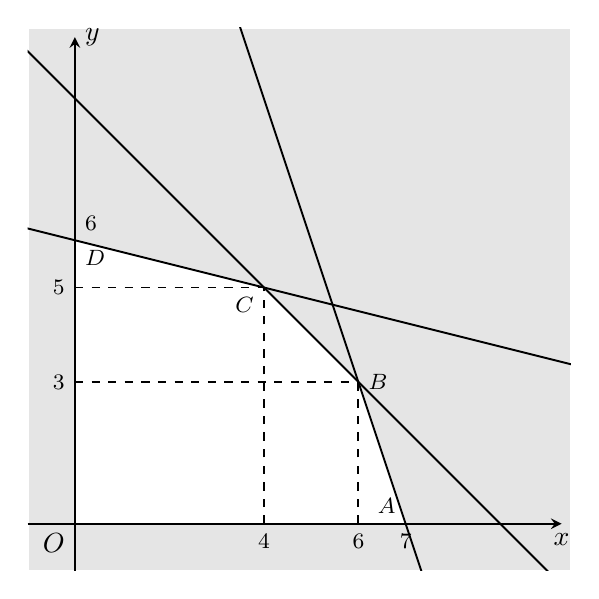
\begin{tikzpicture}[line width=1pt,>=stealth,x=1cm,y=1cm,scale=0.6,line width=0.7pt]
		\clip (-1,-1) rectangle (10.5,10.5);
		\draw[color=white,fill=black!10] (-1,-1) rectangle (10.5,10.5);
		\draw [color=white,fill=white](0,6)--(4,5)--(6,3)--(7,0)--(0,0)--cycle;
		\draw (7,0) node[above left]{\footnotesize$A$};
		\draw (7,0) node[below]{\footnotesize$7$};
		\draw (6,3) node[right]{\footnotesize$B$};
		\draw[dashed] (0,3)--(6,3);
		\draw (0,3) node[left]{\footnotesize$3$};
		\draw[dashed] (6,0)--(6,3);
		\draw (6,0) node[below]{\footnotesize$6$};
		\draw (4,5) node[below left]{\footnotesize$C$};
		\draw[dashed] (0,5)--(4,5);
		\draw (0,5) node[left]{\footnotesize$5$};
		\draw[dashed] (4,0)--(4,5);
		\draw (4,0) node[below]{\footnotesize$4$};
		\draw (0,6) node[below right]{\footnotesize$D$};
		\draw (0,6) node[above right]{\footnotesize$6$};
		\draw[->] (-1,0)--(10.3,0)
		node[below]{$x $};
		\draw[->] (0,-1)--(0,10.3)
		node[right]{$y $};
		\draw (0,0) node[below left]{$ O$};
		\draw[smooth,domain=-5:24] plot (\x,{-3*\x+21});
		\draw[smooth,domain=-5:24] plot (\x,{-\x+9});
		\draw[smooth,domain=-5:24] plot (\x,{-0.25*\x+6});
		\end{tikzpicture}}
		Như vậy để được số điểm thưởng là lớn nhất cần pha chế $ 4 $ lít nước cam và $ 5 $ lít nước táo.\\
		Số điểm thưởng lớn nhất đội nhận được là $4\cdot 60+5\cdot 80=640$ điểm.
	\end{itemchoice}}
\end{ex}
\Closesolutionfile{ans}
\indapan{3}{ans/ans-c2b4-ds}
%---------------Trắc nghiệm trả lời ngắn
\ind{PHẦN III.} \inden{Câu trả lời ngắn.}
\setcounter{ex}{0}
\Opensolutionfile{ans}[ans/ans-c2b4-kq]
\begin{ex}%[0D2H2-1]%[Biên soạn tài liệu dạy học bộ KNTT-CS]%[Trịnh Ngọc Minh]
	Cho hệ bất phương trình $\heva{&x+y-m \geq 0\\&3x+y+2m \geq 0} \quad(\ast)$. Điểm $A(1;1)$ thuộc miền nghiệm của hệ bất phương trình $(\ast)$ khi và chỉ khi $m \in \left[a;b \right]$ với $a$, $b \in \mathbb{R}$. Tính tổng $a+b$.
	\par\shortans[oly]{0}
\loigiai{
	Điểm $A(1;1)$ thuộc miền nghiệm của hệ bất phương trình $(\ast)$ khi và chỉ khi
	\[
	\heva{&1+1-m \geq 0\\&3 \cdot 1+1+2m \geq 0}
	\Rightarrow \heva{&m \leq 2\\&m \geq -2} \Rightarrow m \in [-2;2].
	\]
	Suy ra $a=-2$, $b=2$ nên $a+b=0$.
	}
\end{ex}
\begin{ex}%[0D2H2-2]%[Biên soạn tài liệu dạy học bộ KNTT-CS]%[Trịnh Ngọc Minh]
	\immini[thm]{
	Miền tam giác $ABC$ kể cả ba cạnh sau đây là miền nghiệm của bất phương trình $\heva{&x\ge a\\&bx-4y \le 10\\&4x+cy\le 10}$. Tính $a+b+c$?
	}
	{
	\begin{tikzpicture}[scale=0.7,line join=round, line cap=round,>=stealth]
		\tikzset{label style/.style={font=\footnotesize}}
		\begin{scope}
			\clip (-1,-4) rectangle (3.5,3.5);
			%\draw[color=gray!50,dashed] (-1,-4) grid (5,4);
			\fill[pattern=north west lines,opacity=0.7] (-1,-3.75)--(5,-3.75)--(5,3.75)--cycle;
			\fill[pattern=north west lines,opacity=0.7] (-1,3.75)--(5,3.75)--(5,-2) --(-1,2.8)--cycle;
			\fill[pattern=north west lines,opacity=0.7] (-1,3.75)--(0,3.75)--(0,-3.75)--(-1,-3.75) --cycle;
			\draw (-1,-3.75)--(5,3.75);
			\draw (-1,2.8)--(5,-2);
		\end{scope}
		\node at (0,2.5) [below left]{$A$};
		\node at (0,-2.5) [left]{$C$};
		\node at (2.5,0.5) [above]{$B$};
		\draw[->] (-1,0)--(3.5,0) node[below] {$x$};
		\draw[->] (0,-3.75)--(0,3.5) node[right] {$y$};
		\draw (0,0) node[below left] {$O$};
		\fill (0,2) circle (1pt)node[below right] {$2$};
		\fill (2.5,0) circle (1pt)node[below] {$\tfrac{5}{2}$};
		\foreach \x in {}
		\draw[thin] (\x,1pt)--(\x,-1pt) node [below] {$\x$};
		\foreach \y in {}
		\draw[thin] (1pt,\y)--(-1pt,\y) node [left] {$\y$};
	\end{tikzpicture}
	}
	\par\shortans[oly]{10}
\loigiai{
	Cạnh $AC$ có phương trình $x=0$ và cạnh $AC$ nằm trong miền nghiệm nên $x\ge 0$ là một bất phương trình của hệ.\\
	Cạnh $AB$ qua hai điểm $(0;2)$ và $\left(\dfrac{5}{2};0 \right) $ nên có phương trình $\dfrac{x}{\tfrac{5}{2}}+\dfrac{y}{2} = 1 \Rightarrow 4x+5y =10$.\\
	Điểm $(0;0)$ thuộc miền nghiệm nên $4x+5y\le 10$ là một bất phương trình của hệ.\\
	Suy ra hệ bất phương trình cần tìm là $\heva{&x\ge 0\\&5x-4y \le 10\\&4x+5y\le 10.}$\\
	Vậy $a=0$, $b=5$ và $c=5$.
	}
\end{ex}
\begin{ex}%[0D2H2-2]%[Biên soạn tài liệu dạy học bộ KNTT-CS]%[Trịnh Ngọc Minh]
	Tính diện tích miền nghiệm của hệ bất phương trình $\heva{&x+y\le 4\\ &x\ge 0\\ &y\ge 0.}$
	\par\shortans[oly]{8}
\loigiai{
	\begin{center}
		\begin{tikzpicture}[scale=0.7, font=\footnotesize, line join=round, line cap=round,>=stealth]
			\def \xmin{-1};
			\def \xmax{5};
			\def \ymin{-1};
			\def \ymax{5};
			\draw[->] (\xmin, 0.) -- (\xmax,0.) node[anchor=north] {$x$};
			\draw[->] (0.,\ymin) -- (0.,\ymax) node[anchor=west] {$y$};
			\clip(\xmin-0.1,\ymin-0.1) rectangle (\xmax+0.1,\ymax+0.1);
			\fill[pattern=north east lines,opacity=0.4] (-1,5) plot[smooth,domain=-1:5] (\x,{4-(\x)})--(5,5)--cycle;
			\fill[pattern=horizontal lines,opacity=0.4] (-1,5)-- (0,5)--(0,-1)--(-1,-1)--cycle;
			\draw[smooth] plot[domain=\xmin:\xmax] (\x,{(4-(\x)});
			\fill[pattern=vertical lines,opacity=0.4] (-1,0)--(5,0)--(5,-1)--(-1,-1)--cycle;
			\draw[smooth] plot[domain=\xmin:\xmax] (\x,{(4-(\x)});
			\draw[fill=black] (0,0) circle (1pt) node[below right] {$O$} (1,0) circle(1pt) node[below]{$1$} (2,0) circle(1pt) node[below]{$2$} (3,0) circle(1pt) node[below]{$3$} (4,0) node[below]{$4$} (0,1) circle(1pt) node[left]{$1$} (0,2) circle(1pt) node[left]{$2$} (0,3) circle(1pt) node[left]{$3$} (0,4) circle(1pt) node[left]{$4$};
		\end{tikzpicture}
	\end{center}
	Miền nghiệm là tam giác $OAB$ với $O(0;0)$, $A(4,0)$, $B(0,4)$ là miền nghiệm của hệ bất phương trình.\\
	Vậy $S_{OAB}=\dfrac{1}{2}OA\cdot OB=8$.
	}
\end{ex}
\begin{ex}%[0D2V2-3]%[Biên soạn tài liệu dạy học bộ KNTT-CS]%[Trịnh Ngọc Minh]
	Một hộ nông dân dự định trồng đậu và cà trên diện tích $8$ hecta (ha). Nếu trồng đậu thì cần $20$ công và thu $8$ triệu đồng trên diện tích mỗi ha, nếu trồng cà thì cần $30$ ngày công và thu $10$ triệu đồng trên diện tích mỗi ha. Tính số tiền thu về nhiều nhất, biết rằng tổng số công không quá $180$.
	\par\shortans[oly]{68}
\loigiai{
	Gọi $x$ là số hecta (ha) đất trồng đậu và $y$ là số hecta đất trồng cà. Ta có các điều kiện sau
	\begin{itemize}
		\item $x\ge0$, $y\ge0$.
		\item Diện tích canh tác không vượt quá $8$ ha nên $x+y \le8$.
		\item Số ngày công lao động không vượt quá $180$ ngày nên số ngày công cần trả tiền là
		$20 x+30y \le 180\Leftrightarrow 2 x+3y \le 18$.
	\end{itemize}
	Từ đó, hệ điều kiện ràng buộc $$\heva{&0 \le x \le 8\\&0 \le y \le 8\\&x+y \le 8\\&2x+3y \le18}\quad(1).$$
	\immini{Biểu diễn miền nghiệm của hệ bất phương trình này trên hệ trục toạ độ $Oxy$, ta được miền tứ giác $OABC$ (Hình).\\
	Toạ độ các đỉnh của tứ giác đó là $O(0;0)$; $A(0;6)$; $B(6;2)$; $C(8;0)$.\\
	Gọi $F$ là số tiền (đơn vị: triệu đồng) thu được, ta có $F = 8x +10y$.\\
	Ta phải tìm $x$, $y$ thoả mãn hệ bất phương trình $(I)$ sao cho $F$ đạt giá trị lớn nhất, nghĩa là tìm giá trị
	lớn nhất của biểu thức $F = 8x +10y$ trên miền tứ giác $OABC$.}{\begin{tikzpicture}[scale=.7,>=stealth, font=\footnotesize, line join=round, line cap=round]
	\def\a{1} \def\b{-4} \def\c{3} % Hệ số
	\def\xmin{-.5} \def\xmax{9.5}
	\def\ymin{-.5} \def\ymax{7}
	\draw[color=gray!50,dashed] (\xmin,\ymin) grid (\xmax,\ymax);
	\draw[->] (\xmin,0)--(\xmax,0) node [below]{$x$};
	\draw[->] (0,\ymin)--(0,\ymax) node [left]{$y$};
	\node at (0,0) [below left]{$O$};
	\clip (\xmin+0.1,\ymin+0.1) rectangle (\xmax-0.5,\ymax-0.1);
	\draw[smooth,samples=300,domain=0:9.5] plot(\x,{-1*(\x)+8});
	\draw[smooth,samples=300,domain=0:8.5] plot(\x,{-2/3*(\x)+18/3});
	\draw[fill=black](6,2)node[above]{$B$}circle(1pt)
	(0,6)node[above right]{$A$}circle(1pt)
	(8,0)node[above right]{$C$}circle(1pt)
	;
	\fill[pattern=north east lines,opacity=0.8] (0,0)--(-.5,0)--(-.5,7)--(0,7)--cycle
	(-.5,0)--(-.5,-0.5)--(9,-.5)--(9,0)--cycle
	(0,6)--(0,7)--(9,7)--(9,0)--cycle
	(1,7)--(9,7)--(9,0)--(8,0)--cycle
	;
	\end{tikzpicture}}
	\noindent
	Tính các giá trị của biểu thức $F$ tại các đỉnh của đa giác, ta có tại $O(0;0): F =8\cdot0+ 10\cdot0= 0$; tại $A(0;6):F =8\cdot0+ 10\cdot6= 60$;
	tại $B(6;2):F =8\cdot6+ 10\cdot2= 68$; Tại $C(8;0):F =8\cdot8+ 10\cdot0= 64$.\\
	$F$ đạt giá trị lớn nhất bằng $68$ tại $B(6;2)$.\\
	Vậy bác An thu được nhiều tiền nhất là $68$ triệu đồng.
	}
\end{ex}
\begin{ex}%[0D2V2-3]%[Biên soạn tài liệu dạy học bộ KNTT-CS]%[Trịnh Ngọc Minh]
	Mỗi phân xưởng cần sản xuất ra hai loại sản phẩm. Để sản xuất $1$ kilogam sản phẩm loại I cần sử dụng máy trong $30$ giờ và tiêu tốn $2$ kilogam nguyên liệu. Để sản xuất $1$ kilogam sản phẩm loại II cần sử dụng máy trong $15$ giờ và tiêu tốn $4$ kilogam nguyên liệu. Biết rằng $1$ kilogam sản phẩm loại I thu lãi được $40\,000$ đồng, $1$ kilogam sản phẩm loại II thu lãi được $30\,000$ đồng, có thể sử dụng máy tối đa $1\,200$ giờ và có $200$ kilogam nguyên liệu. Để thu lãi cao nhất, giả sử phân xưởng đó cần sản xuất $x$ kilogam sản phẩm loại I và $y$ kilogam sản phẩm loại II. Tính $x+y$.
	\par\shortans[oly]{$60$}
\loigiai{Ta có bảng
	\begin{center}
		\begin{tabular}{|l|c|c|c|}
			\hline
			\textbf{Sản phẩm} &\textbf{Loại I} &\textbf{Loại II} &\textbf{Tổng}\\
			\hline
			\textbf{Khối lượng sản phẩm} &$x$ &$y$ &$x+y$\\
			\hline
			\textbf{Thời gian sử dụng máy} &$30x$ &$15y$ &$30x+15y\leq 1\,200$\\
			\hline
			\textbf{Khối lượng nguyên liệu} &$2x$ &$4y$ &
			$2x+4y\leq 200$\\
			\hline
			\textbf{Lãi} &$40\,000x$ &$30\,000y$ &$F(x;y)=40\,000x+30\,000y$\\
			\hline
		\end{tabular}
	\end{center}
	Khi đó ta có hệ bất phương trình bậc nhất hai ẩn $\heva{&x\geq 0\\ &y\geq 0\\ &30x+15y\leq 1\,200\\&2x+4y\leq 200} \Rightarrow \heva{&x\geq 0\\ &y\geq 0\\ &2x+y\leq 80\\&x+2y\leq 100.}$\\
	\begin{center}
		\begin{tikzpicture}[line join=round, line cap=round, >=stealth,font=\footnotesize, scale=0.5]
			% Vẽ hệ trục toạ độ
			\draw [->] (-2,0)--(12.5,0) node[above] {$x$};
			\draw[->] (0,-2)--(0,10.5) node[right] {$y$};
			\clip(-2,-2) rectangle (12,10);
			\path (-.6,4.7) node {$50$};
			\path (-.6,4) node {$40$};
			\path (-.6,7.7) node {$80$};
			\path (3.5,-.5) node {$40$};
			\path (2,-.5) node {$20$};
			\path (9.5,-.5) node {$100$};
			\path
			(0,0) coordinate (O)
			(0,5) coordinate (A)
			(2,4) coordinate (B)
			(4,0) coordinate (C)
			;
			\draw[dashed] (0,4)--(2,4)--(2,0);
			%Vẽ đồ thị từng hàm số
			\draw[samples=100,smooth,domain=-2:12] plot(\x,{8-2*(\x)});
			\draw[samples=100,smooth,domain=-2:12] plot(\x,{(10-(\x))/2});
			\draw[samples=100,smooth,domain=-2:10] plot(\x,{0});
			\draw[samples=100,smooth,domain=-2:12] plot({0},\x);
			% Vẽ miền nghiệm
			\fill[opacity=0.4,pattern=north west lines] plot[domain=12:-2](\x,0)--plot[domain=-2:10](\x,{-2})--cycle;
			\fill[opacity=0.4,pattern=north east lines] plot[domain=10:-2](0,\x)--plot[domain=-2:10](-2,\x)--cycle;
			\fill[opacity=0.4,pattern=vertical lines] plot[domain=12:-2](\x,{8-2*(\x)})--plot[domain=-2:12](\x,{10})--cycle;
			\fill[opacity=0.4,pattern=horizontal lines] plot[domain=12:-2](\x,{(10-(\x))/2})--plot[domain=-2:12](\x,{10})--cycle;
			\foreach \x/\g in {O/-135,A/125,B/60,C/-35}{
			\fill (\x) circle (1pt) node[shift=(\g:4mm)] {$\x$};
			}
		\end{tikzpicture}
	\end{center}
	Miền nghiệm của hệ bất phương trình bậc nhất hai ẩn là tứ giác $OABC$ với $O(0;0)$; $A(0;50)$; $B(20;40)$; $C(40;0)$.\\
	Để thu lãi cao nhất thì ta cần $F(x;y)=40\,000x+ 30\,000y$ đạt giá trị lớn nhất. Ta có
	\begin{align*} \allowdisplaybreaks
		&F(0;0)=40\,000 \cdot 0+ 30\,000\cdot 0 = 0;\\
		&F(0;50)=40\,000 \cdot 0+ 30\,000\cdot 50 = 1\,500\,000;\\
		&F(20;40)=40\,000 \cdot 20+ 30\,000\cdot 40 = 2\,000\,000;\\
		&F(40;0)=40\,000 \cdot 40+ 30\,000\cdot 0 = 1\,600\,000.
	\end{align*}
	Vậy thu được lãi cao nhất là $2\,000\,000$ đồng với $x=20$, $y=40$, khi đó $x+y=60$.
	}
\end{ex}
\begin{ex}%[0D2V2-3]%[Biên soạn tài liệu dạy học bộ KNTT-CS]%[Trịnh Ngọc Minh]
	Một công ty sản xuất hai mẫu máy chạy bộ trong nhà. Thời gian lắp ráp hoàn thiện và đóng gói cho mỗi mẫu được mô tả như sau
	\begin{center}
		\begin{tabular}{|c|c|c|c|}
			\hline &Thời gian lắp ráp &Thời gian hoàn thiện &Thời gian đóng gói\\
			&(giờ)&(giờ)&(giờ)\\
			\hline Mẫu A &$3$ &$ 3$ &$0{,}8$\\
			\hline Mẫu B &$4$ &$ 2{,}5$ &$0{,}4$\\
			\hline Thời gian tối đa &$6\,000$ &$ 4\,200$ &$950$\\
			\hline
		\end{tabular}
	\end{center}
	Biết rằng mỗi máy loại $A$ cho lợi nhuận là $3$ triệu đồng, mỗi máy loại $B$ cho lợi nhuận là $3{,}75$ triệu đồng. Khi đó lợi nhận lớn nhất của công ty là bao nhiêu triệu đồng?
	\par\shortans[oly]{5700}
\loigiai{
	Gọi $x$, $y$ lần lượt là số máy loại $A$, $B$ mà công ty sản xuất. Lúc này lợi nhuận là $F(x;y)=3x+3{,}75y$ (triệu đồng).\\
	Ta có hệ điều kiện
	$\heva{&x,y\ge 0\\
	&3x+4y\le 6\,000\\
	&3x+2{,}5y\le 4\,200\\
	&0{,}8x+0{,}4y\le 950.}$\\
	Thu gọn các hệ số ta được hệ bất phương trình\\
	$$\heva{&
	x,y\ge 0\\&
	3x+4y\le 6\,000\\&
	6x+5y\le 8\,400\\&
	2x+y\le 2\,375.
	}
	$$
	Miền nghiệm của hệ là ngũ giác $OABCD$ với $A\left(1\,500;0\right)$ , $B\left(400;1\,200\right)$ , $C\left(868{,}75;637{,}5\right)$ và $D\left(1\,187{,}5;0\right)$\\
	\begin{center}
		\begin{tikzpicture}[>=stealth', x=1cm, y=1cm, scale=1]
			\def\xmin{-2} \def\xmax{5}
			\def\ymin{-2} \def\ymax{4}
			\clip(\xmin,\ymin) rectangle (\xmax,\ymax);
			\tkzDefPoints{\xmax/\ymax/A1,\xmin/\ymax/B1,\xmin/\ymin/C1,\xmax/\ymin/D1}
			\draw[->](\xmin,0)--(\xmax,0); \draw(\xmax-0.1,0) node[below]{$x$};
			\draw[->](0,\ymin)--(0,\ymax); \draw(0,\ymax-0.2) node[right]{$y$};
			\draw[smooth,samples=300] plot(\x,{-0.75*(\x)+3});
			\draw[smooth,samples=300] plot(\x,{-1.22*(\x)+3.41});
			\draw[smooth,samples=300] plot(\x,{-2.02*(\x)+4.79});
			\foreach \ten/\x/\y in {A/0/3,B/0.86/2.35,C/1.75/1.25,D/2.38/0,O/0/0}{
			\coordinate (\ten) at (\x,\y);
			}
			\foreach \p/\r in {A/-70,B/-110,C/180,D/155,O/-120}
			\fill (\p) circle (1pt) node[shift={(\r:3mm)},scale=0.6]{$\p$};
			\fill[pattern=north east lines] (B1)--(0,4)--(0,\ymin)--(C1);
			\fill[pattern=north east lines] (-1.33,4)--(A1)--(D1)--(D)--(C)--(B)--(A);
			\fill[pattern=north east lines] (0,0)--(\xmax,0)--(D1)--(0,\ymin);
			\foreach \p/\r in {1/500,2/1\,000,3/1\,500}
			\fill (0,\p) circle (0.5pt) node[shift={(180:5mm)}]{\small $\r$};
			\foreach \p/\r in {1/500,2/1\,000,3/1\,500}
			\fill (\p,0) circle (0.5pt) node[shift={(-90:5mm)}]{\small $\r$};
		\end{tikzpicture}
	\end{center}
	Ta có
	\begin{itemize}
		\item Tại điểm $A\left(1\,500;0\right)$ thì $F(x;y)= 4\,500$.
		\item Tại điểm $B\left(400;1\,200\right)$ thì $F(x;y)= 5\,700$.
		\item Tại điểm $C\left(868{,}75;637{,}5\right)$ thì $F(x;y)= 4\,996{,}875$.
		\item Tại điểm $D\left(1\,187{,}5;0\right)$ thì $F(x;y)=3\,562,5 $.
		\item Tại điểm $O(0;0)$ thì $F(x;y)= 0$.
	\end{itemize}
	Do đó giá trị lớn nhất của $F(x;y)=F\left(400;1\,200\right)=5\,700$ (triệu đồng).
	}
\end{ex}
\Closesolutionfile{ans}
\indapan{4}{ans/ans-c2b4-kq}
%------------------Tự luận
\ind{PHẦN IV.} \inden{Tự luận.}
\setcounter{ex}{0}
\begin{ex}%[0D2H2-2]%[Biên soạn tài liệu dạy học bộ KNTT-CS]%[Trịnh Ngọc Minh]
	Trong mặt phẳng tọa độ $Oxy$, xét hệ bất phương trình $\heva{&x>0\\&3x+2y<6}$. Biểu diễn miền nghiệm của hệ bất phương trình.
\loigiai{
	\begin{itemize}
		\item Bất phương trình $x>0$ có đường thẳng biên là trục $Oy$.
		\item Bất phương trình $3x+2y<6$ có đường thẳng biên là $d\colon 3x+2y=6$, đi qua hai điểm $A(2;0)$ và $B(0;3)$.
	\end{itemize}
	\begin{center}
		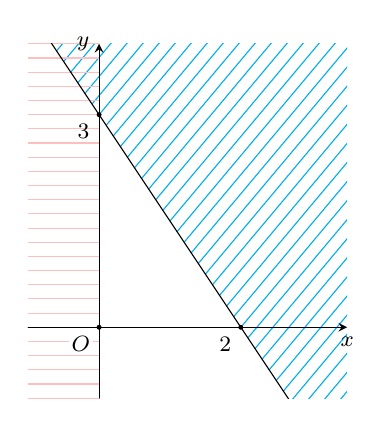
\begin{tikzpicture}[scale=0.9, font=\footnotesize, line join=round, line cap=round, >=stealth] \def\xt{-1} \def\xp{3.5} \def\yt{4} \def\yd{-1} \def\a{1.5} \def\b{3}
			\begin{scope}
				\clip (\xt,\yd) rectangle (\xp,\yt);
				\foreach \x in {-1,-0.9,...,\xp}{\draw[cyan] (\x, \b-\a*\x)--++(50:\xp-\xt);}
				\foreach \y in {-1,-0.8,...,\yt} {\draw[pink] (0,\y)--(\xt,\y);} \fill (0,0) node[below left=2pt, fill=white, inner sep=1pt]{$O$} circle(1pt) (2,0) node[below left]{$2$} circle(1pt) (0,3) node[below left]{$3$} circle(1pt);
				\draw plot[domain=\xt:\xp] (\x,{\b-\a*\x});
			\end{scope}
			\draw[->] (\xt,0)--(\xp,0)node[below]{$x$};
			\draw[->] (0,\yd)--(0,\yt)node[left]{$y$};
		\end{tikzpicture}
	\end{center}
	Miền nghiệm của hệ bất phương trình là phần mặt phẳng không bị gạch bỏ, không kể các đường biên.
	}
\end{ex}
\begin{ex}%[0D2H2-2]%[Biên soạn tài liệu dạy học bộ KNTT-CS]%[Trịnh Ngọc Minh]
	\immini{Phần \textbf{không} tô đậm trong hình vẽ bên (không chứa biên), biểu diễn tập nghiệm của hệ bất phương trình nào?
	}
	{
	\begin{tikzpicture}[line join=round, line cap=round, >=stealth,font=\footnotesize, scale=0.7]
		\draw[->](-2,0)--(3,0) node[below right] {$x$};
		\draw[->](0,-3)--(0,3) node[above] {$y$};
		\clip (-2,-3) rectangle (3,3);
		\node (0,0) [above left]{$ O $};
		\foreach \x in {-1,...,2}
		\draw[shift={(\x,0)},color=black] (0pt,2pt) -- (0pt,-2pt);
		\foreach \y in {-1,...,3}
		\draw[shift={(0,\y)},color=black] (2pt,0pt) -- (-2pt,0pt);
		\draw[samples=100,smooth,domain=-4:2] plot(\x,{(\x)});
		\draw[samples=100,smooth,domain=-4:2] plot(\x,{2*(\x)-1});
		\draw [pattern=north west lines] (3,3)--(-2,3)--(-2,-3)--(-1,-3)--(1,1)--cycle;
		\draw[dashed] (0,1)--(1,1)--(1,0);
		\draw (0,1) node[left]{$1$} (1,0) node[below]{$1$} (0,-1) node[left]{$-1$};
	\end{tikzpicture}
	}
	\loigiai
	{
	\begin{itemize}
		\item Ta thấy biên thức nhất là phân giác của góc phần tư thứ nhất và thứ ba nên có dạng $x-y=0$. Biên thứ hai là đường thẳng $ax+by+c=0$ đi qua $(1;1)$ và $(0;-1)$ nên có dạng $2x-y=1$.
		\item Do miền nghiệm không chứa biên nên các bất phương trình không có dấu\lq\lq=\rq\rq.
		\item Lại có $(1;0)$ thuộc miền nghiệm của hệ bất phương trình.
	\end{itemize}
	Vậy hệ bất phương trình cần tìm có dạng $\heva{&x-y>0\\&2x-y>1.}$
	}
\end{ex}
\begin{ex}%[0D2H2-3]%[Biên soạn tài liệu dạy học bộ KNTT-CS]%[Trịnh Ngọc Minh]
	Bác Ngọc thực hiện chế độ ăn kiêng với yêu cầu mỗi ngày phải hấp thụ tối thiểu $320$ ca-lo, $30$ đơn vị vitamin A và $100$ đơn vị vitamin C. Một cốc đồ uống loại $1$ cung cấp $50$ ca-lo, $12$ đơn vị vitamin A, $10$ đơn vị vitamin C. Một cốc đồ uống loại $2$ cung cấp $60$ ca-lo, $6$ đơn vị vitamin A, $30$ đơn vị vitamin C.
	Gọi $x$, $y$ lần lượt là số cốc loại $1$ và loại $2$ bác Ngọc uống mỗi ngày.
	\begin{enumerate}[a)]
		\item Viết hệ bất phương trình mô tả điều kiện dinh dưỡng.
		\item Nêu hai phương án chọn $(x, y)$ nguyên dương thoả mãn.
	\end{enumerate}
\loigiai{
	\begin{enumerate}[a)]
		\item Theo đề bài ta có hệ bất phương trình
		$\heva{
		&50x + 60y \geq 320 \\
		&12x + 6y \geq 30 \\
		&10x + 30y \geq 100.
		}$
		\item Hai nghiệm thoả mãn đề bài là $(x = 1, y = 5)$; $(x = 2, y = 4)$.
	\end{enumerate}
	}
\end{ex}
\begin{ex}%[0D2H2-2]%[Biên soạn tài liệu dạy học bộ KNTT-CS]%[Trịnh Ngọc Minh]
	\immini{Hệ bất phương trình $\heva{&y-2 x \leq 2\\ &2y-x \geq 4\\ &x+y \leq 5}$ có miền nghiệm là một tam giác như hình vẽ bên. Giá trị nhỏ nhất của biểu thức \mbox{$F(x ;y)=x+3y$} với $(x ;y)$ thỏa mãn hệ bất phương trình trên bằng bao nhiêu?
	}{
	\begin{tikzpicture}[line join=round, line cap=round,>=stealth,thick,scale=0.7]
		\begin{scope}
			\clip (-2,-1) rectangle (6,6);
			\fill[pattern=north east lines,pattern color=red!70] (-3,-4)--(-3,6)--(2,6)--cycle;
			\fill[pattern=north east lines,pattern color=green!70] (-3,0.5)--(-3,-1)--(6,-1)--(6,6)--(8,6)--cycle;
			\fill[pattern=north east lines,pattern color=blue!70] (-1,6)--(6,6)--(6,-1)--cycle;
			\draw[samples=200,domain=-3:2,smooth,variable=\x] plot (\x,{2*(\x)+2});
			\draw[samples=200,domain=-3:8,smooth,variable=\x] plot (\x,{0.5*(\x)+2});
			\draw[samples=200,domain=-1:6,smooth,variable=\x] plot (\x,{-1*(\x)+5});
		\end{scope}
		\draw[->] (-2,0)--(6,0) node[below]{$x$};
		\draw[->] (0,-1)--(0,6) node[left]{$y$};
		\draw (0,0) node[below left]{$O$};
		\foreach \x in {1,2,3,5} \draw[thin] (\x,1pt)--(\x,-1pt) node [below] {$\x$};
		\foreach \x in {-1} \draw[thin] (\x,1pt)--(\x,-1pt) node [above left] {$\x$};
		\foreach \y in {1,2,3,4,5} \draw[thin] (1pt,\y)--(-1pt,\y) node [left] {$\y$};
		\draw[dashed] (2,0)--(2,3) node[above]{$C$}--(0,3) (1,0)--(1,4)node[right]{$B$}--(0,4);
		\draw (0,2) node[below right]{$A$};
	\end{tikzpicture}
	}
\loigiai{
	Tại các đỉnh $A$, $B$, $C$ của miền nghiệm, ta có
	$$F(0;2)=0+3\cdot 2 =6; \quad F(1;4)=1+3\cdot 4=13; \quad F(2;3)=2+3 \cdot 3=11.$$
	Vậy giá trị nhỏ nhất của biểu thức $F(x ;y)=x+3y$ bằng $6$ tại $(0;2)$.
	}
\end{ex}
\begin{ex}%[0D2V2-3]%[Biên soạn tài liệu dạy học bộ KNTT-CS]%[Trịnh Ngọc Minh]
	Người ta dự định dùng hai loại nguyên liệu để chiết xuất ít nhất $140$\,kg chất A và $9$\,kg chất B. Từ mỗi tấn nguyên liệu loại I giá $4$ triệu đồng, có thể chiết xuất được $20$\,kg chất A và $0{,}6$\,kg chất B. Từ mỗi tấn nguyên liệu loại II giá $3{,}5$ triệu đồng, có thể chiết xuất được $10$\,kg chất A và $1{,}5$\,kg chất B. Biết rằng cơ sở cung cấp nguyên vật liệu chỉ có thể cung cấp không quá $10$ tấn nguyên liệu loại I và không quá $9$ tấn nguyên liệu loại II. Giả sử ta dùng $x$ (tấn) nguyên liệu loại I và $y$ (tấn) nguyên liệu loại II để chiết xuất các chất A và B. Chi phí mua nguyên vật liệu (đơn vị: triệu đồng) ít nhất là bao nhiêu?
\loigiai{Ta dùng $x$ (tấn) nguyên liệu loại I và $y$ (tấn) nguyên liệu loại II để chiết xuất các chất A và B thỏa mãn yêu cầu đề bài.\\
	Ta có $\heva{&0 \leq x \leq 10\\ &0 \leq y \leq 9}$.
	Tổng số tiền mua nguyên vật liệu là $T(x;y)=4 x+3{,}5y$ triệu đồng.\\
	Số\,kg chất A chiết xuất được là $20 x+10y \Rightarrow 20 x+10y \geq 140$.\\
	Số\,kg chất B chiết xuất được là $0{,}6 x+1{,}5y \Rightarrow 0{,}6 x+1{,}5y \geq 9$.
	Bài toán đã cho trở thành\\
	Tìm các số $x$ và $y$ thỏa mãn hệ bất phương trình\allowdisplaybreaks
	\begin{eqnarray*}
		\heva{&140 \leq 20 x+10y\\ &9 \leq 0{,}6 x+1{,}5y\\ &0 \leq x \leq 10\\ &0 \leq y \leq 9 } \Leftrightarrow\heva{&14 \leq 2 x+y\\ &30 \leq 2 x+5y\\&0 \leq x \leq 10\\ &0 \leq y \leq 9 }
	\end{eqnarray*} sao cho $T(x;y)=4 x+3{,}5y$ đạt giá trị nhỏ nhất.
	\begin{center}
		\begin{tikzpicture}[font=\footnotesize,line join=round, line cap=round, >=stealth,scale=0.4]
			\tikzset{declare function={x1=-1.5;x2=12.5;y1=-1.5;y2=11.5;
			a=-2;b=14;
			f(\x)=a*(\x)+b;
			a2=-2/5;b2=6;
			g(\x)=a2*(\x)+b2;
			a3=-3/2;b3=27/2;
			h(\x)=a3*(\x)+b3; }}
			\begin{scope}
				\clip (x1,y1)rectangle (x2-.3,y2-.3);
				\draw[smooth,samples=100,domain=x1:x2]plot(\x,{f(\x)});
				\fill[pattern=north west lines,opacity=.5] plot[domain=x1:x2](\x,{f(\x)})--(x1,y1)--(x1,y2);
				\draw[smooth,samples=100,domain=x1:x2]plot(\x,{g(\x)});
				\fill[pattern=north west lines,opacity=.5] plot[domain=x1:x2](\x,{g(\x)})--(x2,y1)--(x1,y1);
				\filldraw[pattern=north west lines,opacity=.5] (x1-.1,9)rectangle(x2,y2);
				\filldraw[pattern=north west lines,opacity=.5] (10,y1-.1)rectangle(x2-.1,y2+.1);
				\filldraw[pattern=north west lines,opacity=.5] (x1-.1,y1-.1)rectangle(x2,0);
				\filldraw[pattern=north west lines,opacity=.5] (x1-.1,y1-.1)rectangle(0,y2);
			\end{scope}
			\draw[->] (x1,0)--(x2,0)node[above]{$x$};
			\draw[->](0,y1)--(0,y2)node[left]{$y$};
			\fill (0,0) circle(1pt) node[shift=(-135:0.25)]{$O$};
			\foreach \x/\goc in {1,2,3,4,5,6,7,8,9,10}{
			\draw (\x,.15)--(\x,-.15)node[below]{$\x$};
			}
			\fill
			(5,4)circle(1pt)node[shift=(30:0.25)]{$A$}
			(10,2)circle(1pt)node[shift=(120:0.25)]{$B$}
			(10,9)circle(1pt)node[shift=(-135:0.25)]{$C$}
			(5/2,9)circle(1pt)node[shift=(20:0.25)]{$D$};
			\foreach \y/\goc in {1,2,3,4,5,6,7,8,9,10}{\draw (.15,\y)--(-.15,\y)node[left]{$\y$};}
		\end{tikzpicture}
	\end{center}
	Ta xác định miền nghiệm $(S)$ của hệ $(*)$ là miền tứ giác $A B C D$ không được gạch chéo như hình vẽ. Trong đó $A(5; 4)$, $B(10; 2)$, $C(10; 9)$, $D\left(\dfrac{5}{2}; 9\right)$.\\
	Biểu thức $T(x;y)$ đạt giá trị nhỏ nhất tại một trong các đỉnh của tứ giác $ABCD$.\\
	Ta có $T(5;4)=34$; $T(10;2)=47$; $T(10;9)=71{,}5$; $T\left(\dfrac{5}{2};9\right)=41{,}5$.\\
	Vậy chi phí mua nguyên vật liệu ít nhất bằng $T(5;4)=34$ triệu đồng.}
\end{ex}
\begin{ex}%[0D2V2-3]%[Biên soạn tài liệu dạy học bộ KNTT-CS]%[Trịnh Ngọc Minh]
	Một xưởng mộc có hai thợ là Chiến và Thắng. Xưởng chuyên sản xuất bàn và ghế. Mỗi bàn bán lãi $500$ nghìn đồng, mỗi ghế bán lãi $400$ nghìn đồng. Để sản xuất được một bàn thì Chiến phải làm việc trong $3$ giờ, Thắng phải làm việc trong $2$ giờ. Để sản xuất được một ghế thì Chiến phải làm việc trong $1$ giờ, Bình phải làm việc trong $4$ giờ. Một người không thể làm được đồng thời bàn và ghế. Biết rằng trong một tháng Chiến không thể làm việc quá $120$ giờ và Bình không thể làm việc quá $200$ giờ. Hỏi số tiền lãi lớn nhất trong một tháng của xưởng là bao nhiêu triệu đồng?
\loigiai{
	\immini{
	Gọi $x$, $y$ lần lượt là số bàn và số ghế được sản xuất ra.
	Điều kiện $x\geq 0$, $y\geq 0$.\\
	Theo giả thiết ta có hệ phương trình $$\heva{&3x+2y\leq 120&\quad(1)&\\&2x+5y\leq 200&\quad(2)&\\&x\geq 0&\quad(3)&\\&y\geq 0&\quad(4)&.}$$
	Miền nghiệm của hệ bất phương trình là tứ giác $OABC$ như hình vẽ. Với $O(0;0)$, $A(0;40)$, $B(40;0)$, $C(8;48)$.
	}
	{
	\begin{tikzpicture}[>=stealth,line join=round,line cap=round,font=\footnotesize,scale=.77,x=.1cm,y=.1cm]
		\def\xmin{-10} \def\xmax{80}
		\def\ymin{-10} \def\ymax{70}
		\path
		(0,50) coordinate (A)
		(40,0) coordinate (B)
		(8,48) coordinate (C)
		;
		\clip (\xmin,\ymin) rectangle (\xmax,\ymax);
		\fill[pattern = north west lines,pattern color = blue!50, smooth,opacity=0.5]
		(\xmax,\ymax)--plot[domain= \xmin:\xmax](\x,{60-(1.5)*\x})-- cycle;
		\fill[pattern = north west lines,pattern color = violet!50, smooth,opacity=0.5]
		(\xmax,\ymax)--(\xmin,\ymax)--plot[domain= \xmin:\xmax](\x,{50-(0.25)*\x})-- cycle;
		\fill[pattern = north west lines,pattern color = green!50, smooth,opacity=0.5]
		(\xmin,\ymin)rectangle(\xmax,0);
		\fill[pattern = north west lines,pattern color = red!50, smooth,opacity=0.5]
		(\xmin,\ymin)rectangle(0,\ymax);
		\foreach \x/\g in
		{A/-120,B/45,C/45}\fill[black]
		(\x) circle (1pt)
		($(\x)+(\g:3mm)$)node{$\x$};
		\draw[->] (\xmin,0)--(\xmax,0) node [above left]{$x$};
		\draw[->] (0,\ymin)--(0,\ymax) node [below right]{$y$};
		\node at (0,0) [above right]{$O$};
		\node at (30,20) [above]{$d_1$};
		\node at (50,38) [above]{$d_2$};
		\draw[color=blue,line width=0.5, smooth, samples=100, domain= -10:110] plot(\x,{60-(1.5)*\x});
		\draw[color=red,line width=0.5, smooth, samples=100, domain= -10:110] plot(\x,{50-(0.25)*\x});
	\end{tikzpicture}}
	Tiền lãi trong một tháng của xưởng là $T=500x+400y$ nghìn đồng.\\
	Ta có $T(A)=16\,000$, $T(B)=20\,000$, $T(C)=23\,200$.\\
	Suy ra $\max T=23\,200$ khi $x=8$ và $y=48$.\\
	Vậy tiền lãi lớn nhất trong một tháng của xưởng là $23\,200\,000$ đồng, tức là $23{,}2$ triệu đồng.
	}
\end{ex}
\Closesolutionfile{ans}